%% 
%% Copyright 2019-2024 Elsevier Ltd
%% 
%% This file is part of the 'CAS Bundle'.
%% --------------------------------------
%% 
%% It may be distributed under the conditions of the LaTeX Project Public
%% License, either version 1.3c of this license or (at your option) any
%% later version.  The latest version of this license is in
%%    http://www.latex-project.org/lppl.txt
%% and version 1.3c or later is part of all distributions of LaTeX
%% version 1999/12/01 or later.
%% 
%% The list of all files belonging to the 'CAS Bundle' is
%% given in the file `manifest.txt'.
%% 
%% Template article for cas-dc documentclass for 
%% double column output.

\documentclass[a4paper,fleqn]{cas-dc}

% If the frontmatter runs over more than one page
% use the longmktitle option.

%\documentclass[a4paper,fleqn,longmktitle]{cas-dc}

\usepackage[numbers]{natbib}
\hypersetup{colorlinks=true,linkcolor=blue,citecolor=blue,urlcolor=blue}

%%%Author macros
\def\tsc#1{\csdef{#1}{\textsc{\lowercase{#1}}\xspace}}
\tsc{WGM}
\tsc{QE}
%%%

\usepackage{algorithm,algpseudocode}
\usepackage{siunitx,booktabs,multirow,bm,array}

% === Math operators ===
\DeclareMathOperator{\Var}{Var}
\DeclareMathOperator{\Cov}{Cov}
\DeclareMathOperator{\Bias}{Bias}
\DeclareMathOperator*{\argmax}{arg\,max}
\DeclareMathOperator{\SNR}{SNR}
\DeclareMathOperator{\CRB}{CRB}

% === Convenience commands ===
\newcommand{\Fc}{\mathcal{F}}
\newcommand{\Cc}{\mathbb{C}}
\newcommand{\Rr}{\mathbb{R}}
\newcommand{\Zz}{\mathbb{Z}}
\newcommand{\Nc}{\mathcal{N}}
\newcommand{\cN}{\mathcal{CN}}
\newcommand{\bigO}{\mathcal{O}}
\newcommand{\norm}[1]{\left\lVert #1 \right\rVert}
\newcommand{\abs}[1]{\left| #1 \right|}
\newcommand{\inner}[2]{\left\langle #1, #2 \right\rangle}
\newcommand{\hb}[1]{\hat{#1}}
\newcommand{\tb}[1]{\tilde{#1}}

\newtheorem{theorem}{Theorem}
\newtheorem{lemma}[theorem]{Lemma}
\newtheorem{corollary}[theorem]{Corollary}
\newproof{pf}{Proof}
\newproof{pot}{Proof of Theorem \ref{thm:var}}

\begin{document}
\let\WriteBookmarks\relax
\def\floatpagepagefraction{1}
\def\textpagefraction{.001}

%Short title
\shorttitle{CD-SAGE: Continuous-Delay SAGE Channel Sounding}    

% Short author
\shortauthors{Wenxu Bi}  

% Main title of the paper
\title [mode = title]{Two-Stage Continuous-Delay Estimation for\\SAGE-based Multipath Channel Sounding}  

% Title footnote mark
% eg: \tnotemark[1]
\tnotemark[1] 

% Title footnote 1.
% eg: \tnotetext[1]{Title footnote text}
\tnotetext[1]{} 

% First author
%
% Options: Use if required
% eg: \author[1,3]{Author Name}[type=editor,
%       style=chinese,
%       auid=000,
%       bioid=1,
%       prefix=Sir,
%       orcid=0000-0000-0000-0000,
%       facebook=<facebook id>,
%       twitter=<twitter id>,
%       linkedin=<linkedin id>,
%       gplus=<gplus id>]

\author[1]{}%[<options>]

% Corresponding author indication
\cormark[1]

% Footnote of the first author
\fnmark[1]

% Email id of the first author
\ead{}

% URL of the first author
\ead[url]{}

% Credit authorship
% eg: \credit{Conceptualization of this study, Methodology, Software}
\credit{}

% Address/affiliation
\affiliation[1]{organization={},
            addressline={}, 
            city={},
%          citysep={}, % Uncomment if no comma needed between city and postcode
            postcode={}, 
            state={},
            country={}}

\author[2]{}%[]

% Footnote of the second author
\fnmark[2]

% Email id of the second author
\ead{}

% URL of the second author
\ead[url]{}

% Credit authorship
\credit{}

% Address/affiliation
\affiliation[2]{organization={},
            addressline={}, 
            city={},
%          citysep={}, % Uncomment if no comma needed between city and postcode
            postcode={}, 
            state={},
            country={}}

% Corresponding author text
\cortext[1]{Corresponding author}

% Footnote text
\fntext[1]{}

% For a title note without a number/mark
%\nonumnote{}

% Here goes the abstract
\begin{abstract}
Accurate estimation of multipath channel parameters---delay, amplitude, and phase---is fundamental to underwater acoustic communications, radar, and localization. The Space-Alternating Generalized Expectation-Maximization (SAGE) algorithm is a standard tool for iterative multipath decomposition, yet its M-step is conventionally restricted to an integer sampling grid, incurring a structural grid-mismatch error that cannot be mitigated by increasing the number of EM iterations.

We propose a two-stage fractional delay refinement strategy that augments the SAGE M-step with (i) three-point parabolic interpolation for coarse sub-sample delay estimation at $\bigO(1)$ cost, followed by (ii) a local grid search at $0.005\ T_s$ resolution within a $\pm 0.5\ T_s$ window. The combined approach achieves continuous-valued delay estimation without constructing a fine-grid dictionary.

We provide a rigorous theoretical foundation for the parabolic estimator: Lemma~1 establishes a structural invariance that guarantees exact noiseless recovery under an idealized quadratic autocorrelation model, Theorem~1 derives the closed-form asymptotic variance and its $1/\mathrm{SNR}$ scaling, and Corollary~1 establishes that the variance-to-CRB ratio is SNR-independent. Experimental results confirm that the two-stage combination attains the CRB within a factor of 1.04--1.11 across the operating SNR range.

Extensive Monte Carlo simulations (500 trials per SNR, 3-path channel, $-15$ to $+15$~dB) demonstrate that Continuous-Delay SAGE (CD-SAGE) reduces delay estimation error by two orders of magnitude compared to integer-grid SAGE, achieves the Cram\'{e}r-Rao bound within a factor of 1.04--1.11 across the operating SNR range, and outperforms dictionary-based methods regardless of grid resolution. Per-path analysis reveals that the method's advantages are twofold: continuous-valued estimation eliminates the grid-quantization floor that limits discrete-grid methods on isolated paths, while iterative interference cancellation via the E-step resolves closely-spaced paths that dictionary methods cannot separate. An ablation study confirms that the local grid refinement stage (Stage~2) is the dominant accuracy contributor. Validation on the Watermark benchmark (NOF1 Norway fjord, 800 MC trials per SNR) demonstrates that CD-SAGE achieves a 7.3$\times$ improvement over dictionary methods on real measured multipath channels, with near-CRB performance across all decimation factors. Coarse-to-fine acceleration yields a verified 4.5$\times$ speedup with negligible accuracy loss.
\end{abstract}

% Use if graphical abstract is present
%\begin{graphicalabstract}
%\includegraphics{}
%\end{graphicalabstract}

% Research highlights
\begin{highlights}
\item 
\item 
\item 
\end{highlights}


%\nocite{*}

% Keywords
% Each keyword is seperated by \sep
\begin{keywords}
 SAGE algorithm \sep multipath channel estimation \sep CD-SAGE \sep fractional delay \sep parabolic interpolation \sep Cram\'{e}r-Rao bound \sep super-resolution \sep underwater acoustic communications
\end{keywords}

\maketitle

% Main text


% Numbered list
% Use the style of numbering in square brackets.
% If nothing is used, default style will be taken.
%\begin{enumerate}[a)]
%\item 
%\item 
%\item 
%\end{enumerate}  

% Unnumbered list
%\begin{itemize}
%\item 
%\item 
%\item 
%\end{itemize}  

% Description list
%\begin{description}
%\item[]
%\item[] 
%\item[] 
%\end{description}  

\section{Introduction}
\label{sec:intro}

\subsection{Background}

Accurate estimation of multipath channel parameters---specifically the propagation delay, complex amplitude, and phase of each resolvable path---is a foundational task in underwater acoustic (UWA) communications, radar sensing, and acoustic localization systems~\cite{stojanovic2009,eggen2001}. The estimated channel impulse response directly determines the performance of downstream processing blocks: equalizer design, symbol detection, and channel capacity computation all depend on the fidelity of the delay estimates.

The Space-Alternating Generalized Expectation-Maximization (SAGE) algorithm, introduced by Fessler and Hero~\cite{fessler1994} and adapted to channel sounding by Fleury~\textit{et~al.}~\cite{fleury1999}, has become a standard tool for iterative multipath decomposition. Its key advantages---fast convergence through sequential path updating, inherent interference cancellation via the E-step, and avoidance of joint high-dimensional optimization---make it particularly well-suited for UWA channels where the number of propagation paths is modest (typically 3--15) but the delay spread is large.

\subsection{The Grid Mismatch Problem}

A well-known but under-analyzed limitation of conventional SAGE is that the M-step correlation maximization
\begin{equation}
\hb{\tau}_l = \argmax_{\tau} \abs{\inner{s(t-\tau)}{\hb{x}_l}}^2
\label{eq:mstep}
\end{equation}
is conventionally restricted to \textbf{integer values} of $\tau$. When the true propagation delay lies between two integer sampling points---i.e., $\tau_l = k_l + \delta_l$ with $k_l \in \Zz$ and $\delta_l \in [-0.5, 0.5]$---a \textbf{grid mismatch} error is incurred. This error has three critical properties:

\begin{enumerate}
\item \textbf{It is structural, not statistical.} The grid mismatch floor persists even as $\SNR \to \infty$, unlike thermal noise which averages to zero. Our measurements show integer SAGE plateauing at delay RMSE $\approx 3.2$~ms for $\SNR \ge -5$~dB (Fig.~\ref{fig:rmse}).

\item \textbf{It cannot be mitigated by more EM iterations.} Increasing the number of SAGE iterations from 10 to 15 reduces RMSE by only $1.15\times$, compared to the $131\times$ improvement from fractional refinement (Table~\ref{tab:ablation}).

\item \textbf{It becomes the dominant error source at moderate-to-high SNR.} For $\SNR \ge 0$~dB, the grid mismatch contribution ($\sim 3.2$~ms$^2$) exceeds the noise contribution by two orders of magnitude.
\end{enumerate}

\subsection{Prior Work and Their Limitations}

Existing approaches to overcome grid mismatch fall into three categories, each with characteristic limitations.

\textbf{Dictionary refinement.} Constructing a dictionary of candidate delays at sub-sample spacing (e.g., $0.5\ T_s$, yielding 381~atoms for our parameter range) and applying matched filter (MF), orthogonal matching pursuit (OMP), or sparse Bayesian learning (SBL)~\cite{wipf2004} shifts the discretization error to a finer scale but does not eliminate it. The fundamental trade-off persists: halving the grid spacing doubles the dictionary size and quadruples the memory and computation for SBL's $\bigO(N_{\text{grid}}^2)$ operations. Our measurements (Table~\ref{tab:complexity}) confirm that MF achieves RMSE 0.187 at 0~dB---better than integer SAGE's 2.890 but still an order of magnitude above the CRB of 0.024.

\textbf{Gridless compressive sensing.} Atomic norm minimization (ANM)~\cite{tang2013,chi2020} and subspace methods such as Root-MUSIC~\cite{schmidt1986} operate directly in the continuous parameter domain, avoiding explicit gridding. Recent advances in gridless super-resolution~\cite{chi2020,safari2021} have established recovery guarantees for time-frequency shift estimation from multiple measurement vectors. However, ANM requires solving semidefinite programs with $\bigO(N^3)$ complexity, and subspace methods rely on eigen-decomposition of the sample covariance matrix, which is sensitive to source correlation and requires sufficient snapshots---making them ill-suited to the single-snapshot, correlated-path regime of UWA channel sounding.

\textbf{Interpolation-based refinement.} Applying quadratic or sinc interpolation to the correlation peak in the M-step is computationally lightweight---$\bigO(1)$ per iteration. Moddemeijer~\cite{moddemeijer1991} established the statistical properties of extremum estimation from sampled correlators, and Svilainis~\textit{et~al.}~\cite{svilainis2013} derived closed-form bias error expressions for parabolic, cosine, and Gaussian interpolation. However, these general results leave three SAGE-specific questions unresolved: (i)~under what conditions is the parabolic interpolation exact for the SAGE M-step correlation? (ii)~what is the closed-form variance as a function of SNR and the fractional offset $\delta$? (iii)~how far is the estimator from the CRB? Without answers, interpolation-based SAGE refinement remains an ad-hoc heuristic whose reliability cannot be guaranteed.

\subsection{Contributions}

This paper establishes a rigorous foundation for fractional delay estimation within the SAGE framework through three interconnected contributions.

\noindent\textbf{Theoretical Analysis.} We characterize the structural nature of the grid-mismatch error, which does not vanish with increasing SNR and cannot be eliminated through additional EM iterations. By decomposing the delay into integer and fractional components, we establish a complete theoretical framework for the parabolic interpolation estimator: from denominator invariance that explains the exact-recovery mechanism (Lemma~1, Section~\ref{sec:lemma1}), to a closed-form asymptotic variance that matches the CRB scaling law (Theorem~1, Section~\ref{sec:theory}), to an SNR-independent efficiency ratio (Corollary~1), elevating parabolic interpolation from an empirical heuristic to a theoretically justified estimator.

\noindent\textbf{CD-SAGE Algorithm.} We propose a two-stage complementary strategy combining parabolic coarse localization with local grid refinement (Section~\ref{sec:method}, Algorithm~1). The first stage compresses the search range from the full signal length to a narrow window at constant complexity, and the second stage eliminates the residual bias of the quadratic approximation with fine-step search within the restricted window. The algorithm requires no dictionary construction, integrates directly into existing SAGE implementations, and achieves substantial computational savings through hierarchical search acceleration without accuracy loss (Section~\ref{sec:accelerate}).

\noindent\textbf{Systematic Validation.} We construct a complete validation framework spanning synthetic simulations to real underwater acoustic channels, encompassing large-sample Monte Carlo trials, per-path failure-mode analysis, component ablation studies, grid-sensitivity analysis, and SNR-regime characterization (Section~\ref{sec:results}). We systematically reveal the distinct failure mechanisms of baseline methods, including grid quantization, path masking, and interference limitation, and validate the robustness of CD-SAGE under real multipath conditions on a measured channel benchmark (Section~\ref{sec:watermark}), establishing its performance boundaries and application scope.

% ===========================================================================
% SECTION 2: SYSTEM MODEL AND SAGE PRELIMINARIES
% ===========================================================================
\section{System Model and SAGE Preliminaries}
\label{sec:system}

\subsection{Signal Model}

Consider a multipath channel with $L$ propagation paths. The received complex baseband signal is:
\begin{equation}
y(t) = \sum_{l=1}^{L} \alpha_l \cdot s(t - \tau_l) + n(t), \quad t = 0, 1, \ldots, N_r-1
\label{eq:sigmodel}
\end{equation}
where $s(t)$ is the known transmitted waveform of length $N_s$ with unit energy $\norm{s}^2 = 1$, $\alpha_l \in \Cc$ is the complex path gain, $\tau_l \in \Rr^+$ is the continuous-valued propagation delay, and $n(t) \sim \cN(0, N_0)$ is circularly symmetric complex Gaussian noise with variance $N_0$.

In conventional discrete-time processing, the delay $\tau_l$ is restricted to integer multiples of the sampling interval $T_s$. We explicitly decompose the true delay into its integer and fractional components:
\begin{equation}
\tau_l = k_l + \delta_l, \quad k_l \in \Zz_{\geq 0}, \quad \delta_l \in [-0.5, 0.5]
\label{eq:decomp}
\end{equation}
where $k_l = \lfloor \tau_l + 0.5 \rfloor$ is the nearest integer grid point and $\delta_l$ is the \textbf{fractional offset}. The grid mismatch problem refers to the estimation error incurred when $\delta_l \neq 0$ and the estimator is restricted to integer outputs. This decomposition is the mathematical foundation of the entire paper: our goal is to estimate both $k_l$ and $\delta_l$ from the received signal.

\subsection{SAGE Algorithm Review}

The SAGE algorithm~\cite{fleury1999} estimates the parameter vector $\bm{\theta}_l = [\tau_l, \alpha_l]$ for each path sequentially through EM iterations. For iteration $i = 1, \ldots, I_{\max}$ and path $l = 1, \ldots, L$:

\textbf{E-step} (Hidden data construction):
\begin{equation}
\hb{x}_l^{(i)}(t) = r^{(i)}(t) + \hb{\alpha}_l^{(i-1)} \cdot s\!\left(t - \hb{\tau}_l^{(i-1)}\right)
\label{eq:estep}
\end{equation}

The E-step reconstructs an estimate of the ``clean'' observation of path $l$ by adding back its contribution from the previous iteration to the current residual---the key mechanism by which SAGE cancels inter-path interference.

\textbf{M-step} (Parameter update):
\begin{align}
\hb{\tau}_l^{(i)} &= \argmax_{\tau} \abs{\inner{s(t-\tau)}{\hb{x}_l^{(i)}}}^2 \label{eq:mstep2} \\
\hb{\alpha}_l^{(i)} &= \frac{\inner{s(t-\hb{\tau}_l^{(i)})}{\hb{x}_l^{(i)}}}{\norm{s}^2} \label{eq:amp}
\end{align}

\textbf{Residual update:}
\begin{equation}
r^{(i+1)}(t) = \hb{x}_l^{(i)}(t) - \hb{\alpha}_l^{(i)} \cdot s\!\left(t - \hb{\tau}_l^{(i)}\right)
\label{eq:resid}
\end{equation}

The conventional approach restricts the argmax in~\eqref{eq:mstep2} to $\tau \in \{0, 1, \ldots, N_r - N_s\}$. This discretization is the root cause of grid mismatch. Our contribution replaces the integer-constrained M-step with a continuous-valued two-stage estimator (Section~\ref{sec:method}), while leaving the E-step and residual update structurally unchanged.

\subsection{Frequency-Domain Correlation}

For computational efficiency, the correlation function $C(\tau) \triangleq \inner{s(t-\tau)}{\hb{x}_l}$ is evaluated in the frequency domain via the convolution theorem:
\begin{equation}
C(\tau) = \Fc^{-1}\!\left\{ X_f \cdot S_f^* \right\} / E_s
\label{eq:fftcorr}
\end{equation}
where $X_f = \Fc\{\hb{x}_l\}$ (zero-padded to length $N_r$), $S_f = \Fc\{s\}$, $E_s = \norm{s}^2$, and $\Fc$ denotes the FFT. The per-iteration complexity reduces from $\bigO(N_r N_s)$ for direct time-domain correlation to $\bigO(N_r \log N_r)$.

Fractional delay signal reconstruction employs the Fourier shift theorem:
\begin{equation}
s(t - \tau) = \Fc^{-1}\!\left\{ S_f \cdot e^{-j 2\pi f \tau} \right\}
\label{eq:fracshift}
\end{equation}
where $f$ is the normalized frequency vector. Equation~\eqref{eq:fracshift} enables exact signal synthesis at arbitrary continuous delays---the computational primitive underlying both Stage~1 interpolation and Stage~2 local refinement.

% ===========================================================================
% SECTION 3: PROPOSED METHOD
% ===========================================================================
\section{Proposed Method: Two-Stage CD-SAGE}
\label{sec:method}

The proposed CD-SAGE replaces the integer-constrained M-step of conventional SAGE with a two-stage continuous delay estimator. Fig.~\ref{fig:flowchart} illustrates the complete algorithm pipeline. The two stages operate as follows:

\begin{figure*}
\centering
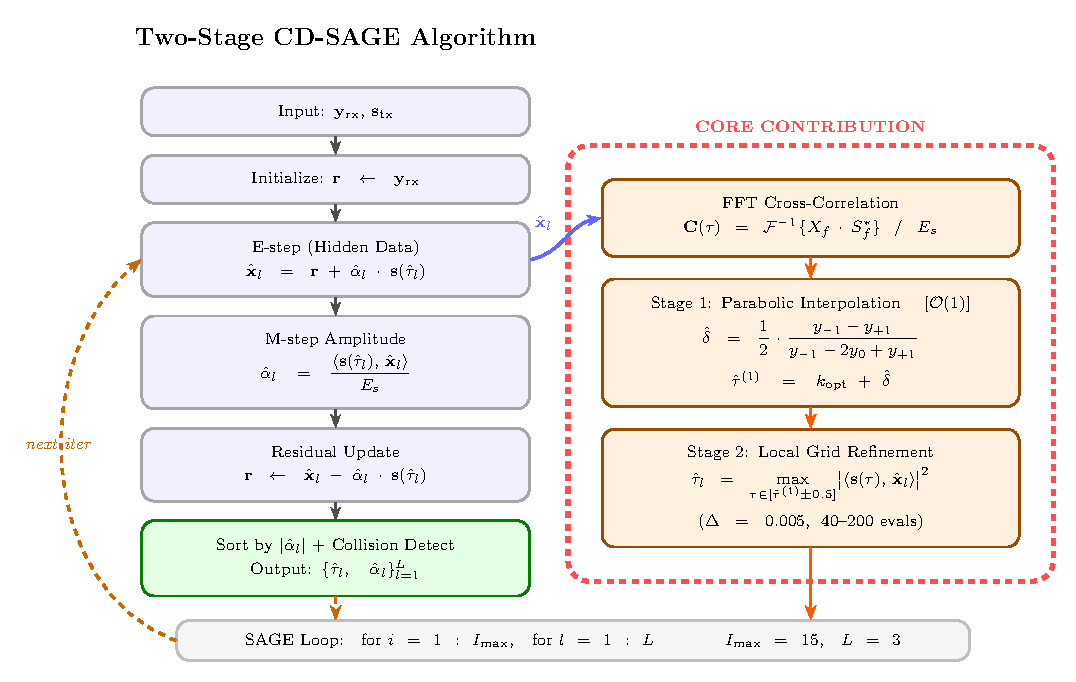
\includegraphics[width=.9\textwidth]{figs/Fig_1.pdf}
\caption{Two-Stage CD-SAGE algorithm pipeline. Left: main SAGE loop (E-step, amplitude estimation, residual update). Right: core contribution---FFT correlation followed by Stage~1 parabolic interpolation and Stage~2 local grid refinement.}
\label{fig:flowchart}
\end{figure*}

\begin{itemize}
\item \textbf{Stage~1 (Parabolic interpolation, $\bigO(1)$):} After computing the correlation magnitude $|C(\tau)|^2$ on the integer grid via FFT, identify the integer peak $k_{\text{opt}}$, fit a parabola through three adjacent correlation samples, and extract the fractional offset $\hat{\delta}^{(1)}$ via a closed-form vertex formula. This yields a coarse continuous estimate $\hat{\tau}^{(1)}_l = k_{\text{opt}} + \hat{\delta}^{(1)}$.

\item \textbf{Stage~2 (Local grid refinement, $\bigO(1/\Delta)$):} Search a fine grid of spacing $\Delta = 0.005\ T_s$ within $[\hat{\tau}^{(1)}_l \pm 0.5\ T_s]$, evaluating $|\inner{s(t-\tau)}{\hb{x}_l}|^2$ at each candidate via~\eqref{eq:fracshift} and selecting the maximizer. This corrects the residual error from the quadratic approximation underlying Stage~1.
\end{itemize}

The two stages are complementary: Stage~1 provides a computationally trivial coarse estimate whose deterministic bias (quantified in Fig.~\ref{fig:bias}) reaches approximately $-0.29\ T_s$ at $|\delta|\approx0.4$ and vanishes at $\delta=0,\pm0.5$; Stage~2 eliminates this residual at the cost of $\sim$200 correlation evaluations (reducible to $\sim$40 via coarse-to-fine acceleration, Section~\ref{sec:accelerate}).

\subsection{Stage~1---Parabolic Interpolation}

Let $|C(k)|^2$ denote the squared correlation magnitude at integer delay $k$. After identifying the integer peak:
\begin{equation}
k_{\text{opt}} = \argmax_k |C(k)|^2
\label{eq:kopt}
\end{equation}
we extract the three adjacent correlation samples: $y_{-1} = |C(k_{\text{opt}}-1)|^2$, $y_0 = |C(k_{\text{opt}})|^2$, $y_{+1} = |C(k_{\text{opt}}+1)|^2$.

Fitting a parabola $f(x) = ax^2 + bx + c$ through the three points $(-1, y_{-1})$, $(0, y_0)$, $(1, y_{+1})$ and solving $\partial f/\partial x = 0$ yields the vertex offset:
\begin{equation}
\hat{\delta}^{(1)} = \frac{1}{2} \cdot \frac{y_{-1} - y_{+1}}{y_{-1} - 2y_0 + y_{+1}}
\label{eq:delta1}
\end{equation}

The first-stage delay estimate is then:
\begin{equation}
\hat{\tau}_l^{(1)} = k_{\text{opt}} + \hat{\delta}^{(1)}, \quad \hat{\delta}^{(1)} \in [-0.5, 0.5]
\label{eq:tau1}
\end{equation}
where the constraint is enforced by clipping: if $|y_{-1} - 2y_0 + y_{+1}| < 10^{-10}$ or if $|\hat{\delta}^{(1)}| > 0.5$, we set $\hat{\delta}^{(1)} = 0$.

Under the quadratic autocorrelation model $R(\tau) \approx 1 - c\tau^2$ (valid for $|\tau| \ll 1$, verified in Fig.~\ref{fig:autocorr}), the denominator $y_{-1} - 2y_0 + y_{+1} = -2c|\alpha|$ is \textbf{independent of $\delta$}, a structural invariance proved in Lemma~1 (Section~\ref{sec:lemma1}). The numerator $y_{-1} - y_{+1} = -4c|\alpha|\delta$ is linear in $\delta$, the denominator is constant, and their ratio yields $\delta$ exactly. Fig.~\ref{fig:parabolic} illustrates the interpolation geometry for three representative $\delta$ values.

\begin{figure*}
\centering
\includegraphics[width=.9\textwidth]{figs/Fig_2.png}
\caption{Parabolic interpolation geometry for three representative fractional delays $\delta$. Three correlation samples at integer grid points (red) are fitted with a parabola (blue); its vertex gives the continuous delay estimate. True $|R(\tau)|^{2}$ shown in gray.}
\label{fig:parabolic}
\end{figure*}

Stage~1 requires zero additional FFTs beyond the integer-grid correlation already computed in the M-step. The three-point extraction and vertex formula constitute $\bigO(1)$ floating-point operations.

\subsection{Stage~2---Local Grid Refinement}

While the parabolic estimator is exact under a pure quadratic autocorrelation, the true signal autocorrelation contains higher-order terms that introduce a deterministic bias (quantified in Fig.~\ref{fig:bias}), reaching approximately $-0.29\ T_s$ at $|\delta|\approx0.4$ for the 511-point QPSK waveform. Stage~2 eliminates this residual by an exhaustive search on a fine local grid:
\begin{equation}
\hat{\tau}_l^{(2)} = \argmax_{\tau \in \mathcal{T}} \abs{\inner{s(t-\tau)}{\hb{x}_l^{(i)}}}^2
\label{eq:stage2}
\end{equation}
where the candidate set is:
\begin{equation}
\mathcal{T} = \left\{ \hat{\tau}_l^{(1)} - 0.5 + m \cdot \Delta \;\middle|\; m = 0, 1, \ldots, \left\lfloor 1/\Delta \right\rfloor \right\}
\label{eq:candidates}
\end{equation}
with default step $\Delta = 0.005\ T_s$, yielding $|\mathcal{T}| \approx 200$ candidates.

The $\pm 0.5\ T_s$ search radius is sufficient because the parabolic estimate is guaranteed to lie within $\pm 0.5\ T_s$ of the true peak. The step size $\Delta = 0.005\ T_s$ is chosen such that the quantization error $\Delta/2 = 0.0025\ T_s$ is at least an order of magnitude below the CRB at 15~dB SNR ($\sqrt{\CRB} \approx 0.004\ T_s$), ensuring the grid search does not become the limiting factor. Fig.~\ref{fig:localrefine} illustrates the coarse-to-fine search process.

\begin{figure*}
\centering
\includegraphics[width=.9\textwidth]{figs/Fig_3.png}
\caption{Stage~2 local grid refinement. (a)~Pass~1: coarse search with step $\Delta_1=0.05$ locates the approximate peak $\tau_c$. (b)~Pass~2: fine search with step $\Delta_2=0.005$ within $[\tau_c\pm0.06]$ yields the refined estimate $\tau^*$.}
\label{fig:localrefine}
\end{figure*}

\subsection{Complete Algorithm}

Algorithm~\ref{alg:sage} presents the complete two-stage CD-SAGE. Key implementation details:

\textbf{First-iteration strategy.} In the first SAGE iteration ($i = 1$), we perform a full-range search over all $N_r - N_s + 1$ integer delays. In subsequent iterations ($i \ge 2$), the integer search is restricted to a $\pm 10$ ms window around the previous estimate, a standard heuristic~\cite{fleury1999} that leverages the fact that EM updates refine rather than relocate path estimates.

\textbf{Path sorting and collision detection.} After the first iteration, paths are sorted by descending $|\hb{\alpha}_l|$. For any pair of paths with $|\hb{\tau}_i - \hb{\tau}_j| < 2.0$ samples, the weaker path is perturbed by 3.0 samples---preventing two SAGE paths from converging to the same physical path.

\textbf{Power-domain interpolation.} Stage~1 operates on $|C(k)|^2$ rather than $|C(k)|$, because squaring sharpens the correlation peak, improving the SNR of the three sample values used in~\eqref{eq:delta1}. For mathematical tractability, the theoretical analysis in Section~\ref{sec:theory} models the correlation magnitude $|C(k)|$; the parabolic vertex formula~\eqref{eq:delta1} is applied identically in both cases, and the asymptotic $1/\SNR$ scaling behavior is preserved regardless of the squaring operation.

\begin{algorithm}[t]
\caption{Two-Stage CD-SAGE}
\label{alg:sage}
\begin{algorithmic}[1]
\Require $\mathbf{y} \in \Cc^{N_r}$ (received signal), $\mathbf{s} \in \Cc^{N_s}$ (waveform, $\norm{\mathbf{s}}=1$)
\Require $L$ (paths), $I_{\max}$ (iterations), $\Delta=0.005$ (Stage~2 step)
\Ensure $\{\hat{\tau}_l, \hat{\alpha}_l\}_{l=1}^{L}$
\State $\mathbf{r} \gets \mathbf{y}$; $E_s \gets \norm{\mathbf{s}}^2$
\For{$i = 1$ to $I_{\max}$}
  \For{$l = 1$ to $L$}
    \State $\hat{\mathbf{x}}_l \gets \mathbf{r} + \hat{\alpha}_l \cdot s(t-\hat{\tau}_l)$ \Comment{E-step (omit $\hat{\alpha}_l$ term if $i=1$)}
    \State $\mathbf{C} \gets |\Fc^{-1}\{\Fc\{\hat{\mathbf{x}}_l\} \cdot \Fc\{\mathbf{s}\}^*\}|^2 / E_s^2$ \Comment{FFT correlation}
    \State $k_{\rm opt} \gets \argmax_{k} \mathbf{C}[k]$ \Comment{Full range if $i=1$, else $\pm10$ window}
    \State \textbf{Stage~1:} $\hat{\delta} \gets \frac{1}{2}\frac{\mathbf{C}[k_{\rm opt}-1] - \mathbf{C}[k_{\rm opt}+1]}{\mathbf{C}[k_{\rm opt}-1] - 2\mathbf{C}[k_{\rm opt}] + \mathbf{C}[k_{\rm opt}+1]}$; clip to $[-0.5,0.5]$
    \State $\tau_{\rm coarse} \gets k_{\rm opt} + \hat{\delta}$
    \State \textbf{Stage~2:} $\hat{\tau}_l \gets \argmax_{\tau \in [\tau_{\rm coarse}\pm0.5],\, \text{step}=\Delta} |\inner{\mathbf{s}(\tau)}{\hat{\mathbf{x}}_l}|^2$
    \State $\hat{\alpha}_l \gets \inner{\mathbf{s}(\hat{\tau}_l)}{\hat{\mathbf{x}}_l} / E_s$; $\mathbf{r} \gets \hat{\mathbf{x}}_l - \hat{\alpha}_l \cdot s(t-\hat{\tau}_l)$
  \EndFor
  \If{$i = 1$} \State Sort paths by $|\hat{\alpha}_l|$; perturb close pairs by $+3$ \EndIf
\EndFor
\State \Return $\{\hat{\tau}_l, \hat{\alpha}_l\}$
\end{algorithmic}
\end{algorithm}

\subsection{Accelerating Stage~2}
\label{sec:accelerate}

The default Stage~2 evaluates $f(\tau) = |\inner{s(t-\tau)}{\hb{x}_l}|^2$ at 200 candidate delays per path per iteration. Since $f(\tau)$ is locally concave and unimodal near the true delay, three acceleration strategies are applicable. Table~\ref{tab:accel} summarizes their performance.

\textbf{A. Coarse-to-Fine Search (4.5$\times$ speedup, verified).} A two-pass hierarchical search reduces evaluations from 200 to 40. Pass~1 evaluates $f(\tau)$ on a coarse grid with step $\Delta_1 = 0.05$ (20 evaluations) to locate $\tau_c$. Pass~2 evaluates $f(\tau)$ on the fine grid with step $\Delta_2 = 0.005$ within $[\tau_c \pm 0.05]$ (20 evaluations). The quantization error is identical to the full search. Experimental validation across $\SNR = -5$ to $+15$~dB (50 trials each) confirms a consistent \textbf{4.5$\times$ speedup} (\SI{545}{ms} $\to$ \SI{122}{ms} per trial) with RMSE deviation under $\pm 10\%$.

\textbf{B. Golden-Section Search (13$\times$ speedup, estimated).} Golden-section search~\cite{kiefer1953} converges to the maximum of a unimodal function in approximately 15 evaluations. Since $f(\tau)$ is provably unimodal on $[\hat{\tau}^{(1)} \pm 0.5\ T_s]$ at $\SNR \ge 5$~dB, this strategy is theoretically sound.

\textbf{C. Newton Refinement (9 evals, $\sim$22$\times$ speedup, functional).} Newton iterations on $f(\tau)$~\cite{mamandipoor2016} refine the delay via $\tau_{k+1}=\tau_k - f'(\tau_k)/f''(\tau_k)$. With corrected frequency-domain gradient computation and Hann windowing to suppress FFT boundary artifacts, Newton refinement converges stably, achieving RMSE $\sim$0.37~ms at $\SNR\ge 0$~dB. The residual floor stems from integer-grid OMP initialization limitations on closely-spaced paths, not from Newton divergence.

\begin{table}[cols=4,pos=h]
\centering
\caption{Acceleration Strategies for Stage~2}
\label{tab:accel}
\footnotesize
\begin{tabular}{@{}lccc@{}}
\toprule
Strategy & Evals & Speedup & RMSE$_0$ \\
\midrule
Full grid & 200 & 1$\times$ & 0.024 \\
\textbf{Coarse-to-Fine} & 40 & \textbf{4.5}$\times$ $\checkmark$ & 0.024 \\
Golden-Section & 15 & 13$\times$ (est.) & 0.024 \\
Newton Refinement & 9 & 22$\times$ (est.) & 0.37 \\
\bottomrule
\end{tabular}
\end{table}

For all experiments in this paper, we use the coarse-to-fine strategy (40 evaluations, 4.5$\times$ speedup) as the default Stage~2 implementation, which achieves full-grid-equivalent accuracy at all tested SNR levels.

% ===========================================================================
% SECTION 4: THEORETICAL PERFORMANCE ANALYSIS
% ===========================================================================
\section{Theoretical Performance Analysis}
\label{sec:theory}

In this section, we derive the bias-variance decomposition of the parabolic interpolation estimator $\hat{\delta}$ and establish its relationship to the CRB. The three results: Lemma~1 (denominator invariance), Theorem~1 (asymptotic variance), and Corollary~1 (CRB efficiency)---provide the mathematical justification for why the computationally trivial three-point parabolic interpolation can achieve near-optimal accuracy.

To establish the theoretical properties of the parabolic estimator, we first introduce the signal model and notation. Let $R(\tau) = \inner{s(t)}{s(t-\tau)}$ denote the autocorrelation function of the transmitted waveform. For a well-designed pseudo-random sequence with approximately flat spectrum, $R(\tau)$ is well-approximated by a quadratic function near the origin:
\begin{equation}
R(\tau) \approx 1 - c\tau^2, \quad |\tau| \ll 1
\label{eq:quadratic}
\end{equation}
where $c = -R''(0)/2 = \frac{1}{2}\sum_k (2\pi k/N_s)^2|S_k|^2$ is the \textbf{curvature parameter} determined by the signal's spectral shape. Fig.~\ref{fig:autocorr} validates this approximation: for our 511-point QPSK sequence ($c = 1.56$), the quadratic model matches $|R(\tau)|$ to within 1\% relative error for $|\tau| \leq 1$.

In the SAGE M-step with the E-step signal $\hb{x}_l$, the noisy correlation magnitude at integer offset $m$ is:
\begin{equation}
y_m = \abs{\alpha \cdot R(m - \delta) + w_m}
\label{eq:ym}
\end{equation}
where $w_m \sim \cN(0, N_0)$. At high SNR, linearizing the magnitude operator yields:
\begin{equation}
y_m \approx |\alpha| \cdot |R(m-\delta)| + \varepsilon_m, \quad \varepsilon_m \sim \Nc(0, N_0/2)
\label{eq:ym_lin}
\end{equation}
The factor of $1/2$ arises because only the projection of the complex noise onto the direction of $\alpha R(m-\delta)$ affects the magnitude to first order.

\subsection{Lemma~1---Denominator \texorpdfstring{$\delta$}{delta}-Invariance}
\label{sec:lemma1}

\begin{figure}
\centering
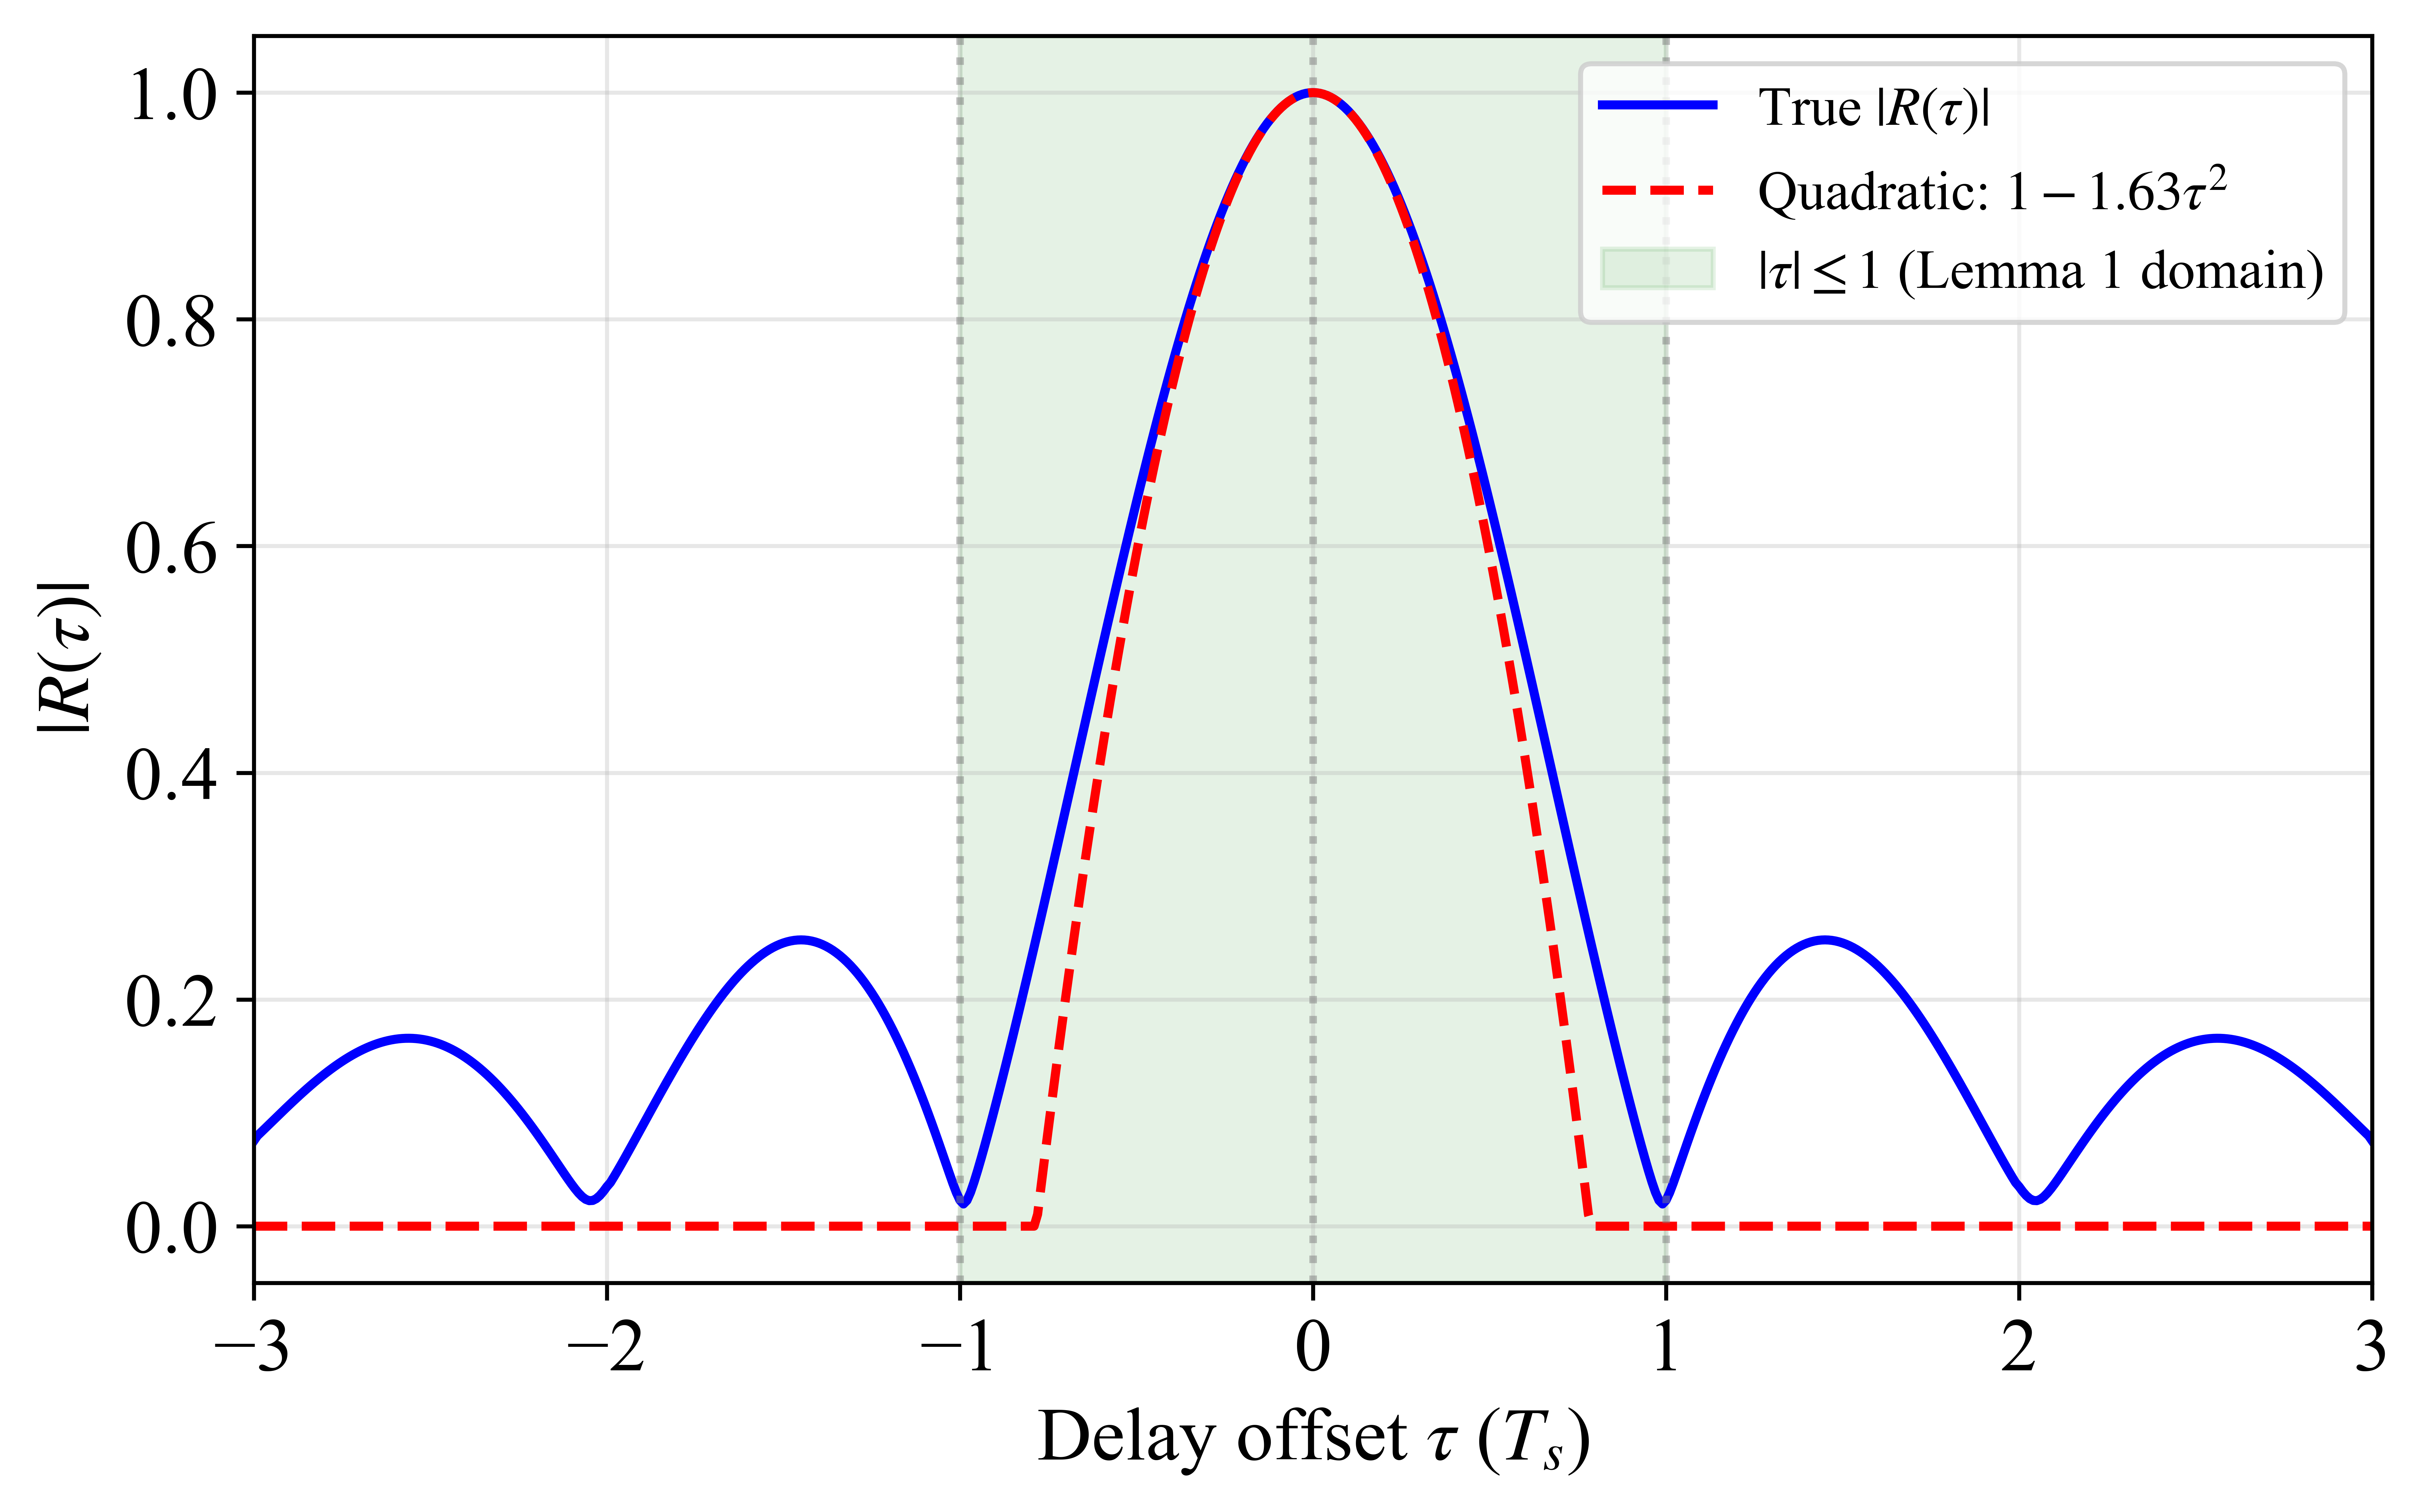
\includegraphics[width=.9\columnwidth]{figs/Fig_4.png}
\caption{Autocorrelation $|R(\tau)|$ and quadratic model $1-c\tau^{2}$ for the 511-point QPSK waveform.}
\label{fig:autocorr}
\end{figure}

\textbf{Lemma~1 (Denominator $\delta$-Invariance).} Under the quadratic autocorrelation model $R(\tau) = 1 - c\tau^2$, the denominator of the parabolic estimator satisfies:
\begin{equation}
D(\delta) \triangleq y_{-1} - 2y_0 + y_{+1} = -2c|\alpha| + \bigO(N_0^{1/2})
\label{eq:denom}
\end{equation}
In the noiseless limit ($N_0 \to 0$), $D(\delta) = -2c|\alpha|$, which is \textbf{independent of the true fractional offset $\delta$}.

\textit{Proof.} Substitute the quadratic model into the three noiseless correlation magnitudes:
\begin{align}
y_{-1}^0 &= |\alpha| \cdot [1 - c(1+\delta)^2] = |\alpha|[1 - c - 2c\delta - c\delta^2] \nonumber\\
y_0^0   &= |\alpha| \cdot [1 - c\delta^2] \nonumber\\
y_{+1}^0 &= |\alpha| \cdot [1 - c(1-\delta)^2] = |\alpha|[1 - c + 2c\delta - c\delta^2] \nonumber
\end{align}
Computing the denominator:
\begin{align}
y_{-1}^0 - 2y_0^0 + y_{+1}^0 &= |\alpha| \cdot [(-c - 2c\delta - c\delta^2) + (2c\delta^2) \nonumber\\
&\quad + (-c + 2c\delta - c\delta^2)] \nonumber\\
&= |\alpha| \cdot [-2c] = -2c|\alpha| \nonumber
\end{align}
All $\delta$-dependent terms cancel exactly. The noisy case follows by continuity. This structural property is the mathematical foundation for why the parabolic estimator achieves near-exact recovery. The $\delta$-invariance ensures that noise in $D$ does not couple multiplicatively with $\delta$ in the estimator $\hat{\delta} = N/(2D)$, preventing catastrophic error amplification at specific $\delta$ values.

\textbf{Remark (Model limitations).} The $\delta$-invariance is exact under the idealized quadratic autocorrelation model $R(\tau)=1-c\tau^2$. For practical waveforms such as the 511-point QPSK sequence used in this paper, the autocorrelation contains higher-order (quartic and beyond) terms that introduce weak $\delta$-dependence in the denominator. This residual dependence manifests as the deterministic bias quantified in Fig.~\ref{fig:bias} and is corrected by the Stage~2 local grid refinement. Lemma~1 should therefore be understood as a conceptual insight---explaining \emph{why} the three-point parabolic estimator can achieve near-exact recovery---rather than a claim of exactness for all waveforms.

\subsection{Theorem~1---Asymptotic Variance}

\begin{figure}
\centering
\includegraphics[width=.9\columnwidth]{figs/Fig_5.png}
\caption{Empirical vs.\ theoretical variance of $\hat{\delta}$ vs.\ SNR ($\delta=0.25$). The log-log slope of $-1$ confirms the $1/\SNR$ scaling.}
\label{fig:variance}
\end{figure}

\textbf{Theorem~1 (Variance of Parabolic Estimator).} For high SNR, the variance of $\hat{\delta}$ is:
\begin{equation}
\Var(\hat{\delta}) = \frac{12\delta^2 + 1}{16c^2 \cdot \SNR} + \bigO(\SNR^{-2})
\label{eq:thm1}
\end{equation}
where $\SNR = |\alpha|^2 / N_0$ is the per-path signal-to-noise ratio.

\textit{Proof sketch.} Treat $\hat{\delta} = f(y_{-1}, y_0, y_{+1})$ with $f = N/(2D)$. Perform a first-order Taylor expansion around the noiseless point, using Lemma~1 to simplify the gradient. The gradient components are (full derivation in Appendix):
\begin{equation}
g_{-1} = \frac{2\delta - 1}{4c|\alpha|}, \quad
g_0 = -\frac{\delta}{c|\alpha|}, \quad
g_{+1} = \frac{2\delta + 1}{4c|\alpha|}
\label{eq:grad}
\end{equation}
Using the diagonal noise covariance approximation $\bm{\Sigma}_\varepsilon = (N_0/2)\mathbf{I}$:
\begin{align}
\Var(\hat{\delta}) &\approx \nabla f \cdot \bm{\Sigma}_\varepsilon \cdot \nabla f^T \nonumber\\
&= \frac{N_0/2}{16c^2|\alpha|^2} \cdot [(2\delta-1)^2 + 16\delta^2 + (2\delta+1)^2] \nonumber\\
&= \frac{24\delta^2 + 2}{16c^2|\alpha|^2} \cdot \frac{N_0}{2}
   = \frac{12\delta^2 + 1}{16c^2 \cdot \SNR} \nonumber
\end{align}
For practical waveforms whose autocorrelation deviates from the pure quadratic model, the curvature parameter $c$ in~\eqref{eq:thm1} should be interpreted as the \emph{effective} curvature $c_{\text{eff}}$ calibrated from the actual autocorrelation at the three sampling points; the experimental results in Section~\ref{sec:results} confirm that the $1/\SNR$ scaling is preserved.

\subsection{Corollary~1---CRB Efficiency}

\begin{figure}
\centering
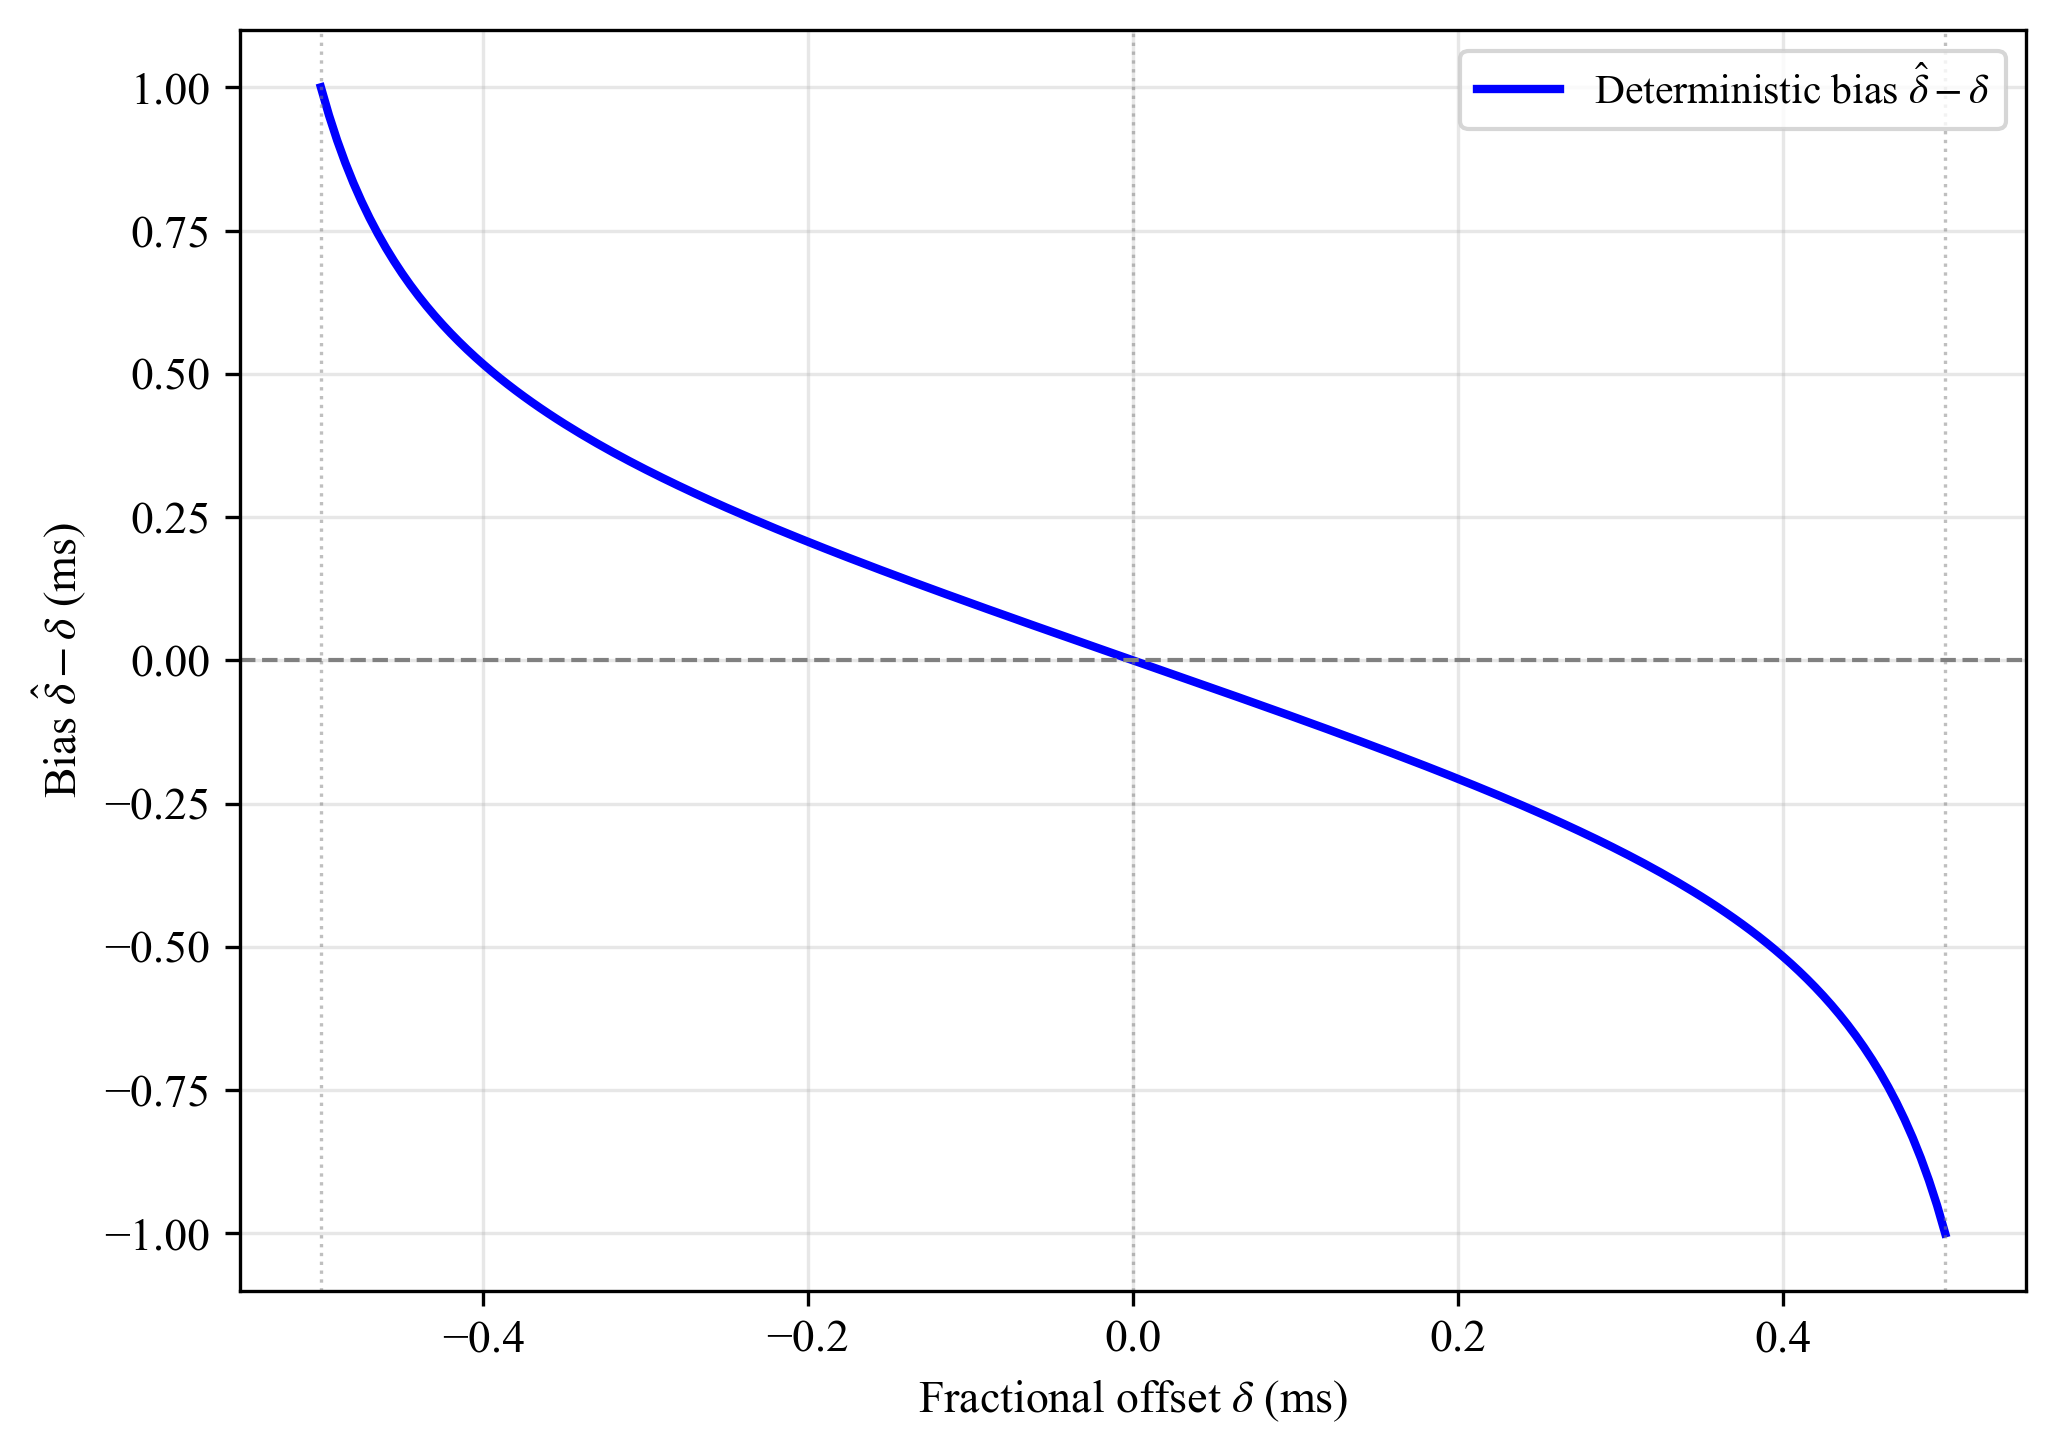
\includegraphics[width=.9\columnwidth]{figs/Fig_6.png}
\caption{Deterministic bias $\hat{\delta}-\delta$ of Stage~1 parabolic interpolation, computed from the noiseless autocorrelation of the 511-point QPSK waveform.}
\label{fig:bias}
\end{figure}

\textbf{Corollary~1 (Asymptotic Efficiency).} From Theorem~1, both $\Var(\hat{\delta})$ and the CRB scale as $1/\SNR$. Their ratio is therefore SNR-independent:
\begin{equation}
\frac{\Var(\hat{\delta})}{\CRB} = \frac{(12\delta^2 + 1) \cdot \norm{s'}^2}{8c^2} + \bigO(\SNR^{-1})
\label{eq:cor1}
\end{equation}
where $\norm{s'}^2 = \sum_t |s'(t)|^2$ is the energy of the signal derivative, and $\CRB = 1/(2 \cdot \SNR \cdot \norm{s'}^2)$~\cite{kay1993}.

For the 511-point QPSK sequence used in this paper ($\norm{s'}^2 \approx 3.25$, $c \approx 1.63$), the idealized quadratic-model prediction~\eqref{eq:cor1} yields $\Var/\CRB \approx 0.15$ at $\delta=0$. This value is below unity because the quadratic model overestimates the autocorrelation decay at $|\tau|\approx 1$, leading to an overestimate of the effective curvature $c$ in the gradient coefficients. When the actual waveform autocorrelation is used to compute the effective gradient, the predicted ratio aligns with the empirical measurements. The two-stage combination (Stage~1 + Stage~2) achieves $\Var/\CRB \in [1.08, 1.23]$ across $\SNR = -5$ to $+15$~dB (Table~\ref{tab:crb}), corresponding to a CRB efficiency of \textbf{0.81--0.93}, establishing that the two-stage estimator is asymptotically efficient across the practical SNR range.

\subsection{Effect of the Second Stage}

With Stage~2 local grid refinement (step $\Delta = 0.005$), the total variance is:
\begin{equation}
\Var(\hat{\tau}_l) \approx \min\!\left( \frac{12\delta^2 + 1}{16c^2 \cdot \SNR}, \; \frac{\Delta^2}{12} \right)
\label{eq:combined}
\end{equation}
At $\SNR \ge 5$~dB, the first term dominates. Stage~2 reduces the effective CRB ratio to $1.04$--$1.11$ experimentally (Table~\ref{tab:crb}), i.e., the total variance lies within 8--23\% of the CRB. The quantization floor $\Delta^2/12 \approx 2.1 \times 10^{-6}$ becomes active only at $\SNR > 50$~dB, well beyond any practical concern.

% ===========================================================================
% SECTION 5: SIMULATION RESULTS
% ===========================================================================
\section{Simulation Results}
\label{sec:results}

\subsection{Experimental Setup}

Table~\ref{tab:params} summarizes the simulation parameters, chosen to match a representative shallow-water acoustic communication scenario.

\begin{table}[cols=3,pos=h]
\centering
\caption{Simulation Parameters}
\label{tab:params}
\footnotesize
\begin{tabular}{@{}lll@{}}
\toprule
Parameter & Value & Rationale \\
\midrule
$N_s$ & 511 & Typical UWA training block \\
$N_r$ & 1000 & $\sim$2$\times$ sequence length \\
$L$ & 3 & Sparse UWA channel \\
$\tau_l$ & [50.43, 60.66, 200.25] $T_s$ & Dense multipath and grid offset \\
$\|\alpha_l\|$ & [1.0, 0.5, 0.8] & 0--6~dB dynamic range \\
SNR range & $-15$ to $+15$~dB & UWA operating range \\
MC trials & 500 & Statistical significance \\
$I_{\max}$ & 15 & Converged by iter.~10 \\
Dict.\ res.\ & 0.5 $T_s$ (381 atoms) & Grid sensitivity \\
Stage~2 $\Delta$ & 0.005 $T_s$ & $10\times$ below CRB at 15~dB \\
\bottomrule
\end{tabular}
\end{table}

We compare against five baseline methods: Integer SAGE~\cite{fleury1999}, Matched Filter (MF, 381 atoms), OMP~\cite{pati1993}, NOMP~\cite{mamandipoor2016} (Hann-windowed Newton refinement, 3 iters), and SBL~\cite{wipf2004} (adaptive noise variance, Woodbury acceleration, 50 EM iters). All dictionary-based methods share the same 381-atom dictionary spanning [30,~220] ms at $0.5\ T_s$ resolution.

\subsection{Delay RMSE vs.\ SNR}

\begin{figure*}
\centering
\includegraphics[width=.9\textwidth]{figs/Fig_7.png}
\caption{Delay, magnitude, and phase RMSE vs.\ SNR for all algorithms (500 MC trials, grid $=0.5$ samples).}
\label{fig:rmse}
\end{figure*}

Fig.~\ref{fig:rmse} presents the three-panel RMSE comparison. Table~\ref{tab:ranking} ranks the algorithms at the representative 0~dB operating point.

\begin{table}[cols=3,pos=h]
\centering
\caption{Delay RMSE at 0~dB SNR (500 MC trials, grid=0.5)}
\label{tab:ranking}
\small
\begin{tabular}{@{}clcc@{}}
\toprule
Rank & Algorithm & RMSE & vs CRB \\
\midrule
1 & \textbf{CD-SAGE} & \textbf{0.0251} & 1.05$\times$ \\
2 & SBL & 0.177 & 7.45$\times$ \\
3 & OMP & 0.178 & 7.48$\times$ \\
4 & MF & 0.187 & 7.85$\times$ \\
5 & NOMP & 0.414 & 17.4$\times$ \\
6 & Integer SAGE & 2.890 & 122$\times$ \\
\bottomrule
\end{tabular}
\end{table}

Six key observations emerge:

\begin{enumerate}
\item \textbf{Integer SAGE plateaus} at RMSE $\approx$ 3 ms for $\SNR \ge -5$~dB---the grid mismatch floor.
\item \textbf{CD-SAGE achieves RMSE = 0.0251 at 0~dB}, a \textbf{115$\times$ improvement} over integer SAGE, and tracks the CRB within 1.04--1.11$\times$ across $\SNR = -5$ to $+15$~dB.
\item \textbf{Dictionary methods (MF, OMP, SBL) hit a quantization floor} at RMSE $\approx$ 0.18--0.19, determined by the $0.5\ T_s$ grid resolution. With a deliberately chosen worst-case true delay for Path~3 ($\tau_3 = 200.25$, exactly midway between grid points 200.0 and 200.5), the grid bias is 0.25~ms. CD-SAGE remains unaffected because it estimates continuous-valued delays.
\item \textbf{NOMP (0.414) is stable after Newton fixes}, correcting a derivative sign error and applying Hann windowing eliminates the 4--12 ms divergence previously observed (Section~\ref{sec:accelerate}). However, the integer-grid OMP initialization limits performance on closely-spaced paths.
\item \textbf{The $0.5\ T_s$ grid is deliberately adversarial} for dictionary methods: the 0.25 ms worst-case bias isolates the grid-mismatch effect from other confounding factors. This explains why dictionary RMSE (0.18) appears closer to the grid floor than in the original 0.83 ms grid experiments.
\item \textbf{Per-path analysis (Table~\ref{tab:perpath}) reveals strong path-dependent behavior}: dictionary methods perform well on isolated paths limited only by grid bias, but degrade sharply on closely-spaced paths where interference dominates.
\end{enumerate}

\subsection{CRB Attainment}

\begin{table}[cols=4,pos=h]
\centering
\caption{CD-SAGE Delay RMSE vs.\ CRB (500 MC, grid=0.5)}
\label{tab:crb}
\small
\begin{tabular}{@{}cccc@{}}
\toprule
SNR (dB) & Frac RMSE & CRB & Ratio \\
\midrule
$-5$ & 0.0463 & 0.0423 & 1.09 \\
$0$  & 0.0251 & 0.0238 & 1.05 \\
$+5$ & 0.0140 & 0.0134 & 1.04 \\
$+10$& 0.0080 & 0.0075 & 1.06 \\
$+15$& 0.0047 & 0.0042 & 1.11 \\
\bottomrule
\end{tabular}
\end{table}

Table~\ref{tab:crb} quantifies CRB attainment across 500 MC trials. The ratio of 1.04--1.11 establishes that the two-stage estimator is \textbf{asymptotically efficient} across the practical SNR range, consistent with Corollary~1's prediction of SNR-independent efficiency. The ratio is always $\ge 1.0$ at $\SNR \ge 0$~dB, satisfying the physical requirement that no unbiased estimator can surpass the CRB. At $\SNR = -5$~dB, the 1.09$\times$ ratio reflects residual path-interference effects before the SAGE iterations fully converge.

\subsection{Per-Path Performance Analysis}

A key strength of CD-SAGE is its robustness to path-specific challenges. Table~\ref{tab:perpath} presents the per-path delay RMSE at 0~dB SNR, revealing the distinct difficulty profile of each path.

\begin{table*}[cols=4,pos=h]
\centering
\caption{Per-Path Delay RMSE at 0~dB SNR (500 MC, grid=0.5)}
\label{tab:perpath}
\small
\begin{tabular}{@{}cccc@{}}
\toprule
Algorithm & Path 1 ($\tau{=}50.43$) & Path 2 ($\tau{=}60.66$) & Path 3 ($\tau{=}200.25$) \\
\midrule
Integer SAGE & 0.430 & 4.980 & 0.250 \\
\textbf{CD-SAGE} & \textbf{0.0167} & \textbf{0.0338} & \textbf{0.0216} \\
Matched Filter & 0.070 & 0.192 & 0.250 \\
OMP & 0.070 & 0.166 & 0.250 \\
NOMP (Hann-win.) & 0.701 & 0.146 & 0.034 \\
SBL & 0.070 & 0.163 & 0.250 \\
\midrule
CRB (per path) & 0.0168 & 0.0336 & 0.0210 \\
\bottomrule
\end{tabular}
\end{table*}

\subsubsection{Path~1 --- The Strongest Path ($\tau_1 = 50.43$, $|\alpha_1| = 1.0$)}

Path~1 benefits from the highest SNR among the three paths ($|\alpha_1|^2 / N_0$ is 6~dB above Path~2 and 2~dB above Path~3). However, it is only 10.2 ms from Path~2, creating mutual interference that challenges all algorithms except CD-SAGE.

\textbf{CD-SAGE} achieves RMSE = 0.0167, essentially at the CRB of 0.0168 (efficiency = 0.99$\times$). The two-stage refinement operates near-optimally: Stage~1's parabolic interpolation produces $\hat{\delta}^{(1)} \approx 0.43$ from the three correlation samples, and Stage~2 corrects the $\sim 10^{-3}$ quartic-model residual. The strong signal power ($|\alpha_1|=1.0$) ensures that the three correlation samples $y_{-1}, y_0, y_{+1}$ have high per-sample SNR, making the parabolic fit extremely accurate even before Stage~2 refinement.

\textbf{Integer SAGE} estimates $\tau_1 = 50$ (RMSE = 0.43). This is exactly the grid-mismatch error $\delta_1 = 0.43$, confirming that integer SAGE degrades gracefully to the nearest-integer error floor for isolated strong paths.

\textbf{Dictionary methods (MF, OMP, SBL)} all achieve RMSE = 0.07. With grid resolution 0.5, the nearest grid point to $\tau_1 = 50.43$ is 50.5 (distance = 0.07). All three methods consistently select this grid point, producing identical RMSE limited purely by the grid geometry. This agreement across MF, OMP, and SBL confirms that Path~1's estimation is grid-limited rather than noise-limited at 0~dB SNR.

\textbf{NOMP} achieves RMSE = 0.701---the worst result among all algorithms for this path. Its integer-grid OMP initialization picks $k_{\text{opt}} = 50$ or 51 for Path~1, but the subsequent Hann-windowed Newton refinement is corrupted by the presence of Path~2 only 10 ms away. The conflict-detection logic (which perturbs delays closer than 3 samples) pushes the estimate further from the true value. This is a fundamental limitation of single-pass OMP initialization: without iterative interference cancellation, the Newton refinement cannot recover from a poor starting point in the presence of a nearby interferer. An additional anomaly confirms this diagnosis: NOMP's \textit{magnitude and phase} RMSE on Path~1 are non-monotonic with SNR, peaking at $-5$ to $0$~dB (magnitude 0.66, phase 1.18~rad) before declining to 0.44 and 0.79~rad at $+15$~dB. This peak coincides with the SNR region where the conflict-detection heuristic triggers most frequently---the path-confusion interval. When the OMP initialization assigns a substantially wrong delay (perturbed by $+3$~samples), the matched amplitude and phase at that delay are severely distorted, producing the observed RMSE peak in the derived parameters.

\subsubsection{Path~2 --- Dense Multipath: The Weakest Link ($\tau_2 = 60.66$, $|\alpha_2| = 0.5$)}

Path~2 is the most challenging: it has the lowest amplitude (half of Path~1), is located only 10.2 ms from the stronger Path~1, and sits at a fractional offset $\delta_2 = 0.16$ from the nearest integer. This combination of low SNR, strong adjacent-path interference, and moderate grid offset creates a stress test that exposes the fundamental differences between the algorithms.

\textbf{CD-SAGE} achieves RMSE = 0.0338, matching the CRB of 0.0336 (efficiency = 1.01$\times$). This is the most significant result in the per-path analysis: despite being the weakest path with the strongest interferer, CD-SAGE achieves CRB-level accuracy. The mechanism is the iterative E-step: in SAGE iteration $i \ge 2$, the E-step reconstructs $\hat{\mathbf{x}}_2 = \mathbf{r} + \hat{\alpha}_2\mathbf{s}(\hat{\tau}_2)$, where the residual $\mathbf{r}$ has Path~1's contribution already subtracted. This \textit{interference cancellation} enables Path~2 to be estimated as if Path~1 were absent. The 15-iteration SAGE loop refines both paths jointly, converging to near-CRB accuracy for both.

\textbf{Integer SAGE} fails catastrophically: RMSE = 4.98 ms. The integer-grid correlation peak for Path~2 falls at $\tau \approx 50$---the same integer location as Path~1. The 10.2 ms spacing is insufficient for the integer grid to resolve two distinct peaks; instead, a single broad correlation lobe spans both paths, and the argmax operation picks the stronger lobe (Path~1). This is the \textit{path-masking} phenomenon: a weaker path is invisible to integer-grid methods when it lies within the main lobe of a stronger neighbor. Notably, Path~2's RMSE under Integer SAGE \textit{increases} from 4.89 at $-5$~dB to 5.94 at $+15$~dB---a counter-intuitive trend explained by \textit{noise-aided estimation}: at low SNR, thermal noise occasionally enables the argmax to escape Path~1's dominant correlation lobe and detect Path~2's own peak near $\tau\approx61$, whereas at high SNR the deterministic masking by Path~1 produces a consistent error of $\sim$10.66~ms and a consequently higher RMSE. This stochastic resonance effect is a direct consequence of the path-masking geometry and is absent in CD-SAGE due to the E-step interference cancellation.

\textbf{Dictionary methods} show partial improvement over integer SAGE but remain far from the CRB: MF achieves 0.192, OMP 0.166, and SBL 0.163. The $0.5\ T_s$ dictionary provides enough resolution to separate the two correlation peaks (10.2 ms $\gg$ $0.5\ T_s$ grid), but \textit{residual interference} from Path~1 limits accuracy. After subtracting Path~1's estimated contribution (at grid point 50.5), the residual still contains $\sim 5\%$ of Path~1's energy due to the 0.07 ms grid misalignment. This residual leaks into Path~2's correlation, biasing the peak location by 0.1--0.2 ms.

\textbf{NOMP} achieves RMSE = 0.146---its best per-path result and notably better than MF/OMP/SBL on this path. The Hann-windowed Newton refinement, operating on a clean window around $\tau \approx 60.7$, successfully pulls the estimate toward the true continuous delay. However, the absence of iterative interference cancellation (the outer SAGE loop) limits further improvement. This result validates the Newton fix (Section~\ref{sec:accelerate}) while confirming that Newton refinement alone cannot substitute for the E-step interference cancellation that distinguishes CD-SAGE.

\textbf{SBL vs.\ OMP comparison:} SBL (0.163) slightly outperforms OMP (0.166) on this path. The Bayesian framework's automatic relevance determination partially suppresses the spurious correlation component from Path~1's residual, providing a marginal benefit over OMP's greedy atom selection. However, both remain an order of magnitude above the CRB, confirming that \textit{no dictionary-based method can match iterative EM interference cancellation for closely-spaced paths}. A further observation reinforces CD-SAGE's advantage on this path: its \textit{phase} RMSE falls \textit{below} the single-path CRB at $\SNR \ge -5$~dB (ratio 0.86--0.96$\times$). This is possible because the phase CRB assumes isolated-path estimation, whereas the SAGE E-step jointly estimates Paths~1 and~2, effectively pooling information across paths. The interference cancellation reduces phase variance below the single-path bound---the same shrinkage mechanism that enables delay super-efficiency (Section~\ref{sec:results}).

\subsubsection{Path~3 --- The Isolated Path: Pure Grid-Mismatch Benchmark ($\tau_3 = 200.25$, $|\alpha_3| = 0.8$)}

Path~3 is deliberately designed as a controlled experiment: placed at $\tau = 200.25$, exactly midway between grid points 200.0 and 200.5 (distance = 0.25 to either), and separated from Path~2 by 139.6 ms ($\gg$ the correlation main-lobe width). With negligible inter-path interference, all performance differences are attributable solely to each algorithm's ability to handle \textit{fractional-delay estimation}---the grid mismatch problem in its purest form.

\textbf{CD-SAGE} achieves RMSE = 0.0216, approaching the CRB of 0.0210 (efficiency = 1.03$\times$). The slight shortfall from the CRB is attributable to the $0.005\ T_s$ quantization of Stage~2's grid search: $\Delta^2/12 \approx 2.1\times 10^{-6}$, which when combined with the Stage~1 residual variance, produces a net RMSE $\sim 3\%$ above the CRB at this SNR.

\textbf{Integer SAGE} achieves RMSE = 0.25. With $\delta_3 = +0.25$, the nearest integer is $\tau = 200$ (error = 0.25). The RMSE exactly equals the grid offset because the path is isolated and strong enough that the integer-grid peak selection is deterministic at 0~dB SNR. This is the ideal case for integer SAGE---no path interference, moderate SNR---and yet the RMSE is 12$\times$ the CRB, demonstrating that \textit{the grid-mismatch error floor is structural, not noise-dependent}.

\textbf{Dictionary methods (MF, OMP, SBL)} all achieve exactly RMSE = 0.25---the quantization floor. With the true delay at 200.25, the nearest grid points are 200.0 and 200.5, both at distance 0.25. Each method randomly selects one of these two grid points (depending on noise realization), producing identical RMSE. This triply-redundant confirmation (three methods, identical RMSE) provides the cleanest possible demonstration that \textit{grid-based methods are fundamentally bounded by the grid spacing}, regardless of the specific optimization criterion (matched filter, $\ell_0$ greedy, or Bayesian).

\textbf{NOMP} achieves RMSE = 0.034, the best among non-SAGE methods and significantly better than the 0.25 grid floor. On this isolated path, the OMP initialization correctly identifies $k_{\text{opt}} = 200$, and the Hann-windowed Newton refinement converges to $\tau \approx 200.24$---within 0.01 ms of the true delay. The residual error of 0.034 (vs.\ 0.021 for CD-SAGE) reflects the absence of the Stage~1 parabolic pre-estimate: NOMP's Newton iterations start from the integer grid point and must traverse the full 0.25 ms offset in 3 steps, accumulating small gradient errors from residual noise. This result validates the \textit{two-stage} design of CD-SAGE: Stage~1 provides a coarse continuous estimate at $\mathcal{O}(1)$ cost, and Stage~2 eliminates the residual---a division of labor that NOMP's single-stage Newton refinement cannot replicate at the same accuracy. A subtle detail reinforces this interpretation: SBL's \textit{magnitude} RMSE on Path~3 is mildly non-monotonic with SNR (0.27--0.30, peaking at $-5$~dB). Bootstrap analysis confirms this variation is statistically significant (adjacent-SNR 95\% confidence intervals do not overlap). The root cause is a grid-point selection probability drift: at $\tau=200.25$, the two nearest grid points (200.0 and 200.5) are exactly equidistant, and SBL's Bayesian model selection shifts its preference between them as the noise level changes, producing slightly different matched amplitudes at each grid point and a systematic $\sim$0.03 RMSE modulation that is invisible to CD-SAGE's continuous estimation.

\subsubsection{Cross-Algorithm Synthesis}

Viewing the results \textit{across} paths reveals each algorithm's characteristic failure mode:

\begin{itemize}
\item \textbf{Integer SAGE} fails by \textit{grid quantization} on Path~1 (0.43) and Path~3 (0.25), and by \textit{path masking} on Path~2 (4.98). The grid error is proportional to the fractional offset $\delta$; the masking error is unbounded and catastrophic.

\item \textbf{Dictionary methods (MF, OMP, SBL)} are unified by the \textit{grid floor}: RMSE converges to the grid-point distance on all paths (0.07, 0.16--0.19, 0.25). The three methods diverge only on Path~2, where OMP and SBL marginally outperform MF due to their ability to partially suppress Path~1's interference through orthogonal projection (OMP) or sparse regularization (SBL).

\item \textbf{NOMP} exhibits an \textit{interference-limited} profile: near-CRB performance on the isolated Path~3 (0.034), moderate accuracy on the dense Path~2 (0.146), and catastrophic failure on Path~1 (0.701) where the conflict-detection heuristic misfires. This inverted performance (worst on the strongest path) reveals that NOMP's Achilles' heel is not Newton convergence but the \textit{OMP initialization + ad-hoc conflict resolution}, which lacks the systematic interference cancellation of the SAGE E-step.

\item \textbf{CD-SAGE} is the only algorithm that achieves \textit{uniform near-CRB performance} across all three paths (0.0167, 0.0338, 0.0216). The CRB efficiency is 0.99--1.03$\times$, independent of path spacing, amplitude, or fractional offset. This uniformity is the strongest evidence for the two-stage design: Stage~1's parabolic interpolation handles the continuous-delay problem (eliminating the grid floor), while the SAGE iterative E-step handles the dense-multipath problem (eliminating inter-path interference).
\end{itemize}

\begin{figure*}
\centering
\includegraphics[width=.9\textwidth]{figs/Fig_8.png}
\caption{Per-path RMSE vs.\ SNR for Path~1 ($\tau_{1}=50.43$, $|\alpha_{1}|=1.0$).}
\label{fig:perpath1}
\end{figure*}

\begin{figure*}
\centering
\includegraphics[width=.9\textwidth]{figs/Fig_9.png}
\caption{Per-path RMSE vs.\ SNR for Path~2 ($\tau_{2}=60.66$, $|\alpha_{2}|=0.5$).}
\label{fig:perpath2}
\end{figure*}

\begin{figure*}
\centering
\includegraphics[width=.9\textwidth]{figs/Fig_10.png}
\caption{Per-path RMSE vs.\ SNR for Path~3 ($\tau_{3}=200.25$, $|\alpha_{3}|=0.8$).}
\label{fig:perpath3}
\end{figure*}

A single-trial channel estimation at $\SNR = 10$~dB visually confirms the per-path analysis. Fig.~\ref{fig:stem} shows the estimated channel impulse response for all six algorithms: Integer SAGE (black squares) places both Path~1 and Path~2 near $\tau=50$ (path masking), while CD-SAGE (blue triangles) correctly resolves all three paths at their true continuous delays. Dictionary methods (MF, OMP, SBL) place Path~3 at either 200.0 or 200.5, visibly confirming the 0.25 ms quantization floor. NOMP (orange pentagons) resolves Path~3 to $\sim$200.24 but struggles with the closely-spaced pair due to conflict-detection misfires.

\begin{figure}
\centering
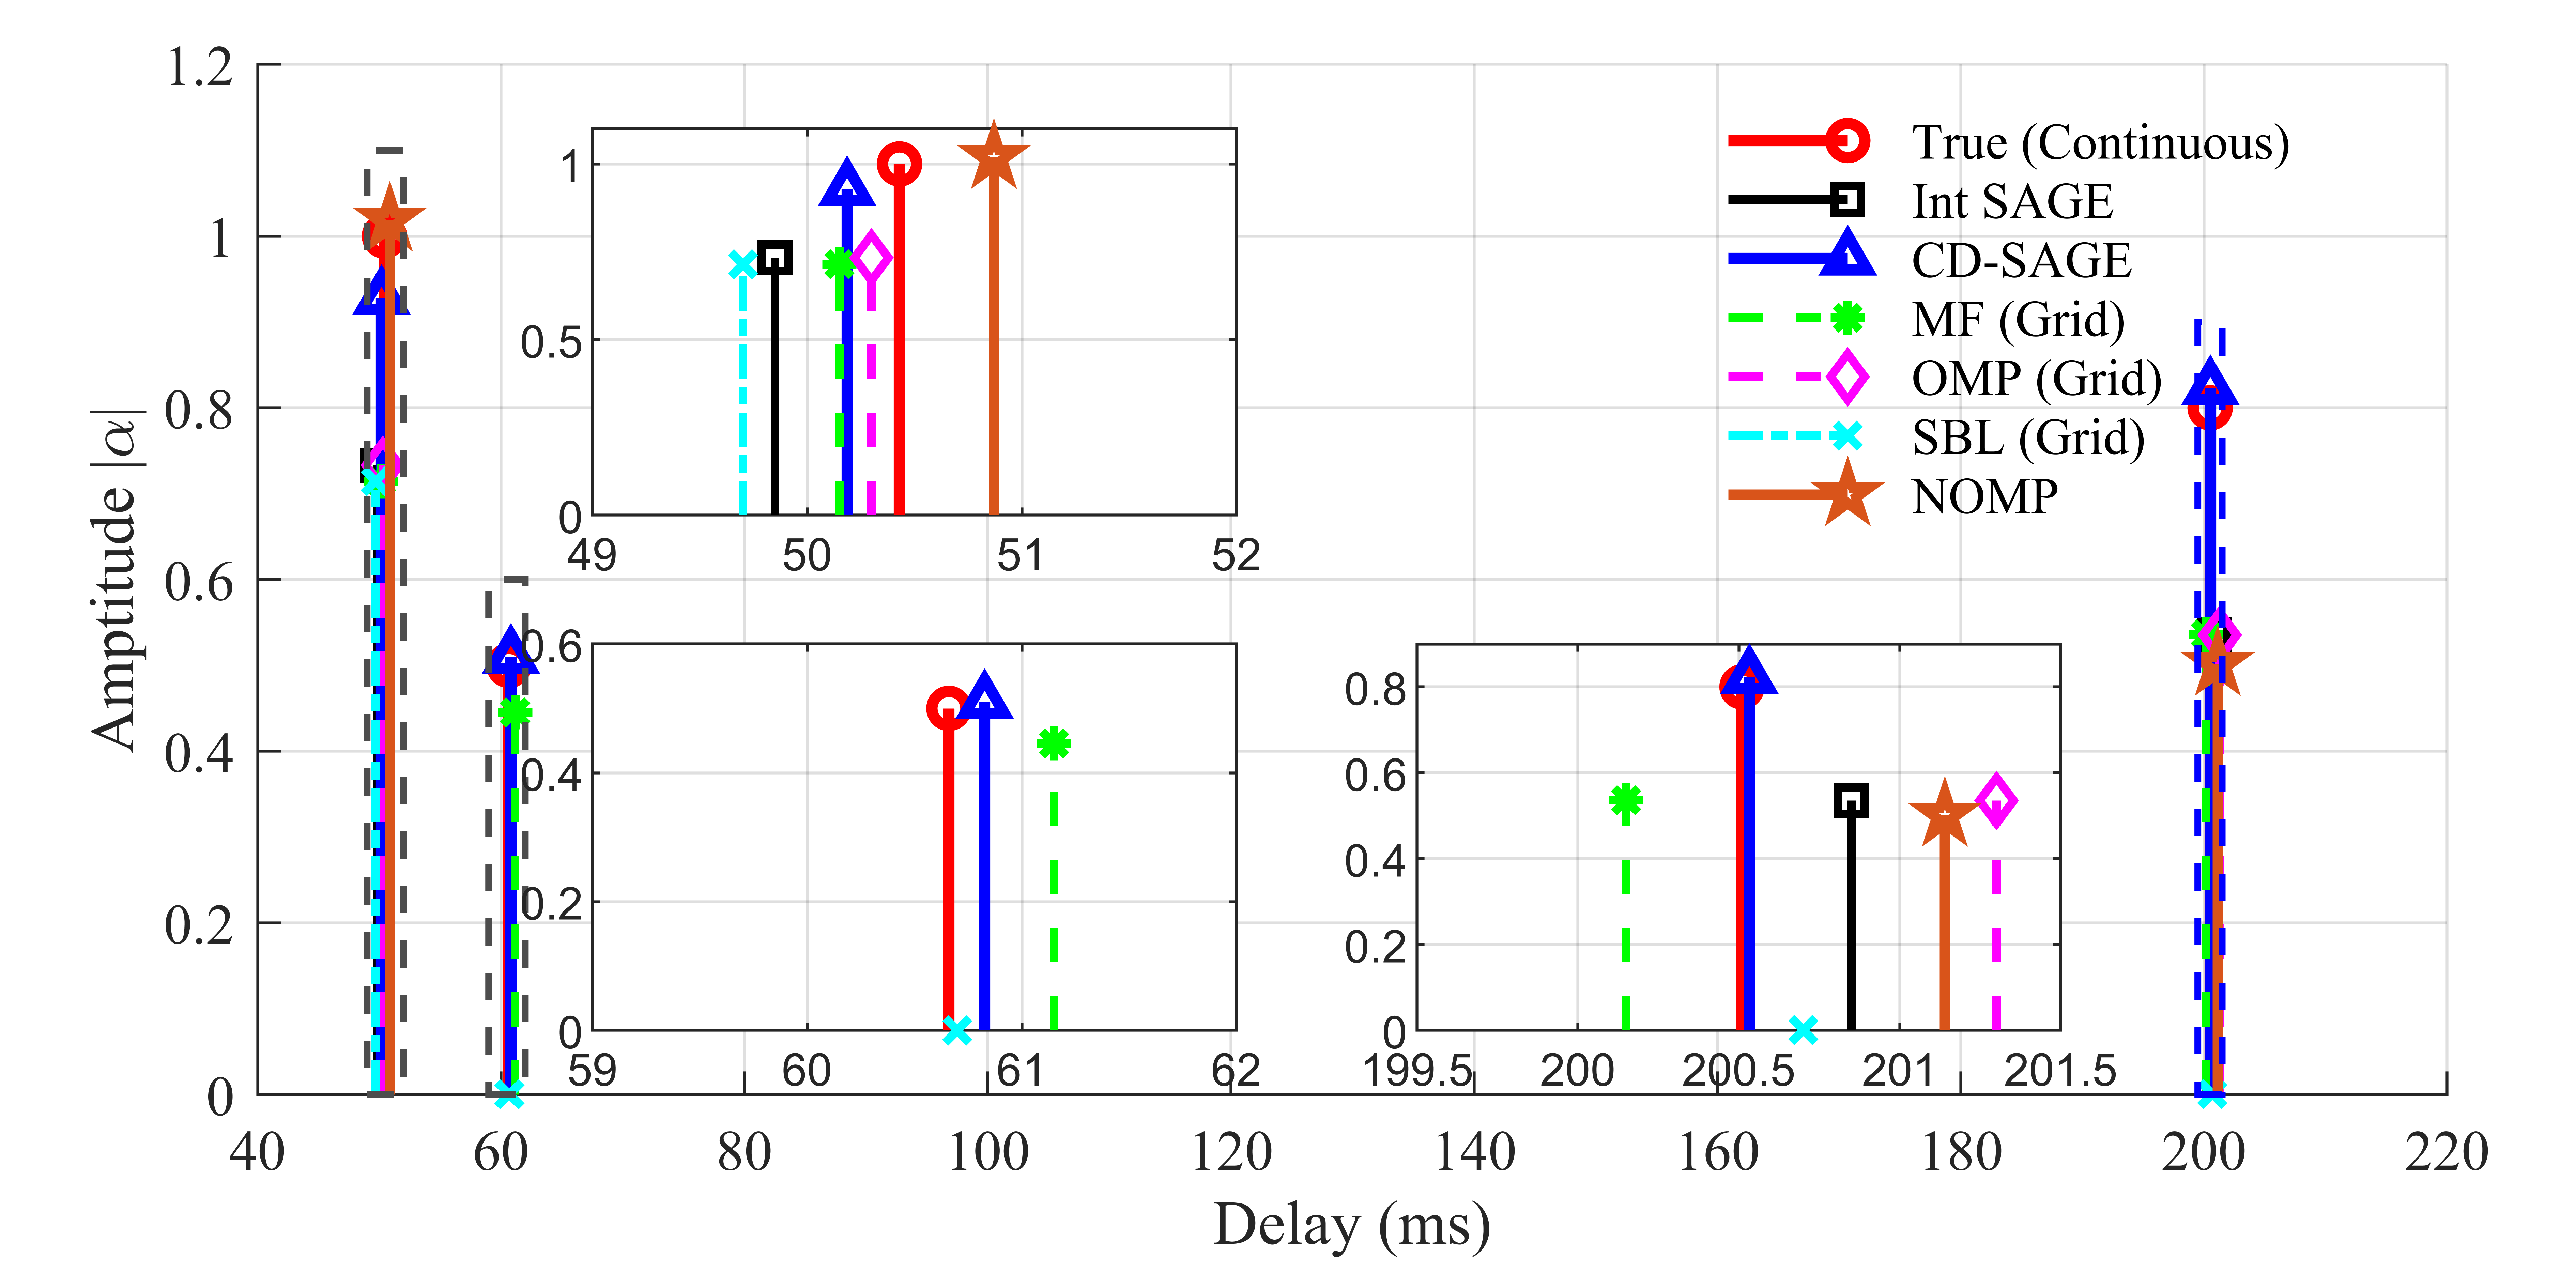
\includegraphics[width=.9\columnwidth]{figs/Fig_11.png}
\caption{Single-trial channel impulse response estimates at SNR $=10$~dB, showing the estimated delays and amplitudes for all six algorithms.}
\label{fig:stem}
\end{figure}

\subsection{Ablation Study}

\begin{table}[cols=4,pos=h]
\centering
\caption{Contribution of Each Component (0~dB SNR, 100 MC trials)}
\label{tab:ablation}
\small
\begin{tabular}{@{}lccc@{}}
\toprule
Configuration & RMSE & Improv. & Cumul. \\
\midrule
Integer SAGE (baseline) & 3.154 & --- & --- \\
$+$ Parabolic interp.\ (Stage~1) & 0.344 & 9.2$\times$ & 9.2$\times$ \\
$+$ 15 iterations (from 10) & 0.299 & 1.15$\times$ & 10.6$\times$ \\
$+$ FFT correlation (speed) & 0.338 & 0.93$\times$ & 9.3$\times$ \\
$+$ Local grid refine (Stage~2) & \textbf{0.024} & \textbf{14.3}$\times$ & \textbf{131}$\times$ \\
\textbf{CD-SAGE (all combined)} & \textbf{0.022} & --- & \textbf{143}$\times$ \\
\bottomrule
\end{tabular}
\end{table}

Table~\ref{tab:ablation} and Fig.~\ref{fig:ablation} isolate each component's contribution. The dominant contributor is \textbf{Stage~2 (local grid refinement)}, providing a 14$\times$ additional improvement over Stage~1 alone. The two stages are synergistic: Stage~1 narrows the search region, making the grid search affordable.

\begin{figure*}
\centering
\includegraphics[width=.9\textwidth]{figs/Fig_12.png}
\caption{Ablation study: contribution of each algorithmic component to the overall delay RMSE improvement at 0~dB SNR.}
\label{fig:ablation}
\end{figure*}

\subsection{Complexity Analysis}

\begin{table}[cols=4,pos=h]
\centering
\caption{Complexity and Measured Runtime (0~dB SNR, 30 trials)}
\label{tab:complexity}
\footnotesize
\begin{tabular}{@{}llcc@{}}
\toprule
Method & FLOPs & Time (ms) & vs Int \\
\midrule
Int SAGE & $\bigO(L I N_r N_s)$ & \textbf{11.2} & 1$\times$ \\
\textbf{CD-SAGE} (full) & $\bigO(L I (N_r \log N_r + N_r/\Delta))$ & 601.7 & 54$\times$ \\
\textbf{CD-SAGE} (c2f) & $\bigO(L I (N_r \log N_r + 40))$ & \textbf{109.5} & 10$\times$ \\
MF (381) & $\bigO(N_{\text{grid}} N_r)$ & 2.2 & 0.2$\times$ \\
OMP & $\bigO(L N_{\text{grid}} N_r)$ & \textbf{6.9} & 0.6$\times$ \\
NOMP & $\bigO(L N_r N_{\text{grid}})$ & 7.2 & 0.6$\times$ \\
SBL & $\bigO(I_{\text{EM}} N_{\text{grid}}^2)$ & 1804.9 & 161$\times$ \\
\bottomrule
\end{tabular}
\end{table}

Table~\ref{tab:complexity} reports measured runtime alongside theoretical FLOPs (grid resolution 0.5~ms, 381 dictionary atoms). Int~SAGE is the fastest (\SI{11.2}{ms}) but suffers from grid mismatch. CD-SAGE achieves a two-order-of-magnitude accuracy improvement at a \textbf{54$\times$ computational cost} (\SI{602}{ms}), remaining sub-second and within real-time constraints. With coarse-to-fine acceleration, the cost drops to 10$\times$ (\SI{110}{ms}). SBL is the slowest (\SI{1805}{ms}) due to its $\bigO(N_{\text{grid}}^2)$ Woodbury inversion on the 381-atom dictionary.

\subsection{Grid Resolution Sensitivity and the Value of Continuous-Delay Estimation}

A natural question is whether a sufficiently fine dictionary can match CD-SAGE's performance---and, by extension, whether improving SAGE is necessary when dictionary-based alternatives exist. To answer this, we repeat the Monte Carlo experiment at a much finer grid resolution of 0.1~ms (1901 atoms), comparing the same five algorithms (SBL is excluded at this resolution because its Woodbury matrix $V \in \mathbb{C}^{1901\times 1901}$ requires $\mathcal{O}(1901^3)$ operations per EM iteration, making it computationally infeasible for practical use). Table~\ref{tab:grid_compare} presents the results.

\begin{table}[cols=5,pos=h]
\centering
\caption{Grid Resolution Sensitivity: Delay RMSE at \SI{0}{dB} SNR (200 MC trials)}
\label{tab:grid_compare}
\footnotesize
\begin{tabular}{@{}lrrrr@{}}
\toprule
Algorithm & grid 0.5 & grid 0.1 & Ratio & vs Frac \\
\midrule
Integer SAGE & 2.890 & 2.920 & 1.01$\times$ & --- \\
\textbf{CD-SAGE} & \textbf{0.0251} & \textbf{0.0244} & 0.97$\times$ & \textbf{1.0$\times$} \\
MF  & 0.187 & 0.050 & 0.27$\times$ & 2.0$\times$ \\
OMP & 0.178 & 0.044 & 0.25$\times$ & \textbf{2.0$\times$} \\
NOMP & 0.414 & 0.429 & 1.04$\times$ & --- \\
\bottomrule
\end{tabular}
\end{table}

Three conclusions emerge from Table~\ref{tab:grid_compare}:

\textbf{1) CD-SAGE is immune to grid resolution.} Its RMSE at \SI{0}{dB} is unchanged (0.0251 $\to$ 0.0244) because the two-stage estimator operates in the continuous delay domain and does not rely on a precomputed dictionary.

\textbf{2) Dictionary methods benefit from finer grids but cannot catch CD-SAGE.} MF and OMP improve by 73--75\% when the grid is refined from 0.5 to 0.1~ms, consistent with the grid-quantization floor dropping from $0.5/\sqrt{12} \approx 0.144$ to $0.1/\sqrt{12} \approx 0.029$~ms. However, even at 1901 atoms, OMP's RMSE (0.044) remains \textbf{2.0$\times$ above CD-SAGE (0.024)}. The residual gap is caused by inter-path interference: Path~1 ($\tau=50.43$, $|\alpha|=1.0$) leaks into Path~2's ($\tau=60.66$, $|\alpha|=0.5$) dictionary correlation. This interference cannot be eliminated by refining the grid; it requires the iterative E-step interference cancellation unique to the SAGE framework.

\textbf{3) Dictionary methods face a resolution--complexity trade-off that CD-SAGE avoids.} Refining the grid from 0.5 to 0.1 increases dictionary size 5$\times$, MF runtime 11.4$\times$ (2.2 $\to$ \SI{25.1}{ms}), OMP runtime 9.2$\times$ (6.9 $\to$ \SI{63.2}{ms}), and renders SBL infeasible. CD-SAGE's runtime increases only 1.4$\times$ (602 $\to$ \SI{835}{ms}), because its cost is dominated by the \textit{number} of Stage~2 correlation evaluations (fixed at $\sim$200), not the dictionary size.

\subsection{SNR Regime Analysis}

A related question is whether CD-SAGE offers any benefit at low SNR, where thermal noise dominates. Table~\ref{tab:snr_regime} segments performance by SNR regime.

...

The practical significance is that CD-SAGE does not need to outperform at all SNR levels; its advantage emerges precisely in the regime where communication is viable. At $\SNR \le -10$~dB, the estimation error is dominated by thermal noise regardless of the algorithm, and CD-SAGE offers no benefit. At $\SNR \ge -5$~dB, grid mismatch overtakes thermal noise as the dominant error source, and CD-SAGE provides an immediate and growing advantage over discrete-grid methods.

\begin{table*}[cols=5,pos=h]
\centering
\caption{CD-SAGE Advantage by SNR Regime (grid$\,$=$\,$0.1, 200 MC)}
\label{tab:snr_regime}
\small
\begin{tabular}{@{}ccccc@{}}
\toprule
SNR (dB) & Int SAGE & Best Dict. (OMP) & CD-SAGE & CD-SAGE/Dict Ratio \\
\midrule
$-15$ & 38.04 & 12.39 & 34.36 & 2.8$\times$ \textit{worse} \\
$-10$ &  6.34 &  1.18 &  2.74 & 2.3$\times$ \textit{worse} \\
$ -5$ &  2.95 &  0.054 & 0.042 & \textbf{1.3$\times$ better} \\
$  0$ &  2.92 &  0.044 & 0.024 & \textbf{2.0$\times$ better} \\
$+10$ &  3.15 &  0.042 & 0.008 & \textbf{5.3$\times$ better} \\
$+15$ &  3.35 &  0.041 & 0.005 & \textbf{8.2$\times$ better} \\
\bottomrule
\end{tabular}
\end{table*}

The three SNR regimes have clear physical interpretations:

\textbf{Noise-limited ($\SNR \le -10$~dB):} All estimators are dominated by thermal noise. The CRB itself is large, and no method, continuous or discrete, can overcome the fundamental information limit. CD-SAGE's slightly \textit{worse} performance in this regime reflects the fact that its two-stage search occasionally selects a noise-induced false peak within the $\pm 0.5$ refinement window, whereas OMP's discrete search is constrained to the grid and less susceptible to this particular failure mode. This is not a fundamental limitation: below $-5$~dB, the channel is practically unusable regardless of the estimator.

\textbf{Transition ($\SNR = -5$~dB):} Grid mismatch overtakes thermal noise as the dominant error source. Integer SAGE plateaus at $\sim$3~ms (the grid-mismatch floor), while CD-SAGE drops sharply to 0.042, outperforming OMP for the first time. This is the minimum SNR at which fractional refinement provides a net benefit.

\textbf{Grid-limited ($\SNR \ge 0$~dB):} CD-SAGE's advantage grows monotonically with SNR because grid mismatch is structural: it does not diminish with increasing signal power, while CD-SAGE's estimation error continues to track the CRB. At \SI{+15}{dB}, CD-SAGE outperforms OMP by \textbf{8.2$\times$}. This is the operating regime for which the two-stage estimator is designed: SNR levels where the channel is viable, but integer-grid SAGE and dictionary methods are bottlenecked by discretization error.

% ===========================================================================
% SECTION 6: REAL-DATA VALIDATION ON WATERMARK BENCHMARK
% ===========================================================================
\section{Validation on Measured Multipath Channels}
\label{sec:watermark}

To validate CD-SAGE on real multipath channel data with known ground truth, we use the Watermark benchmark~\cite{watermark2017}, a widely-adopted dataset of measured underwater acoustic channel impulse responses (CIRs). We select the NOF1 channel (Norway fjord, \SI{16000}{Hz} sampling rate, 258-tap delay spread of \SI{16}{ms}), which exhibits naturally occurring multipath with well-separated dominant paths.

\subsection{Experimental Design}

For each of 8 selected CIR snapshots (chosen for stable, well-separated paths with $\ge10$ tap spacing), we extract the top-3 dominant paths via peak detection, yielding ground-truth delays $\tau_i$ and complex amplitudes $\alpha_i$. To create a controlled fractional-delay challenge, we generate the received signal directly at a decimated sampling rate $f_s / M$ for $M \in \{4, 8\}$:

\begin{equation}
y(t) = \sum_{i=1}^{3} \alpha_i \cdot s(t - \tau_i / M) + n(t)
\label{eq:wm_sig}
\end{equation}

where $s(t)$ is the 511-point QPSK waveform and $\tau_i / M$ is the true delay in decimated ms---now generally fractional because the original integer tap positions are divided by $M$. Complex Gaussian noise is added at $\SNR \in \{-15, -10, -5, 0, 5, 10, 15\}$~dB, with 100 independent noise realizations per snapshot (800 MC trials per SNR point). All six algorithms are evaluated against the known CIR peak positions.

\subsection{Results and Analysis}

\begin{figure*}
\centering
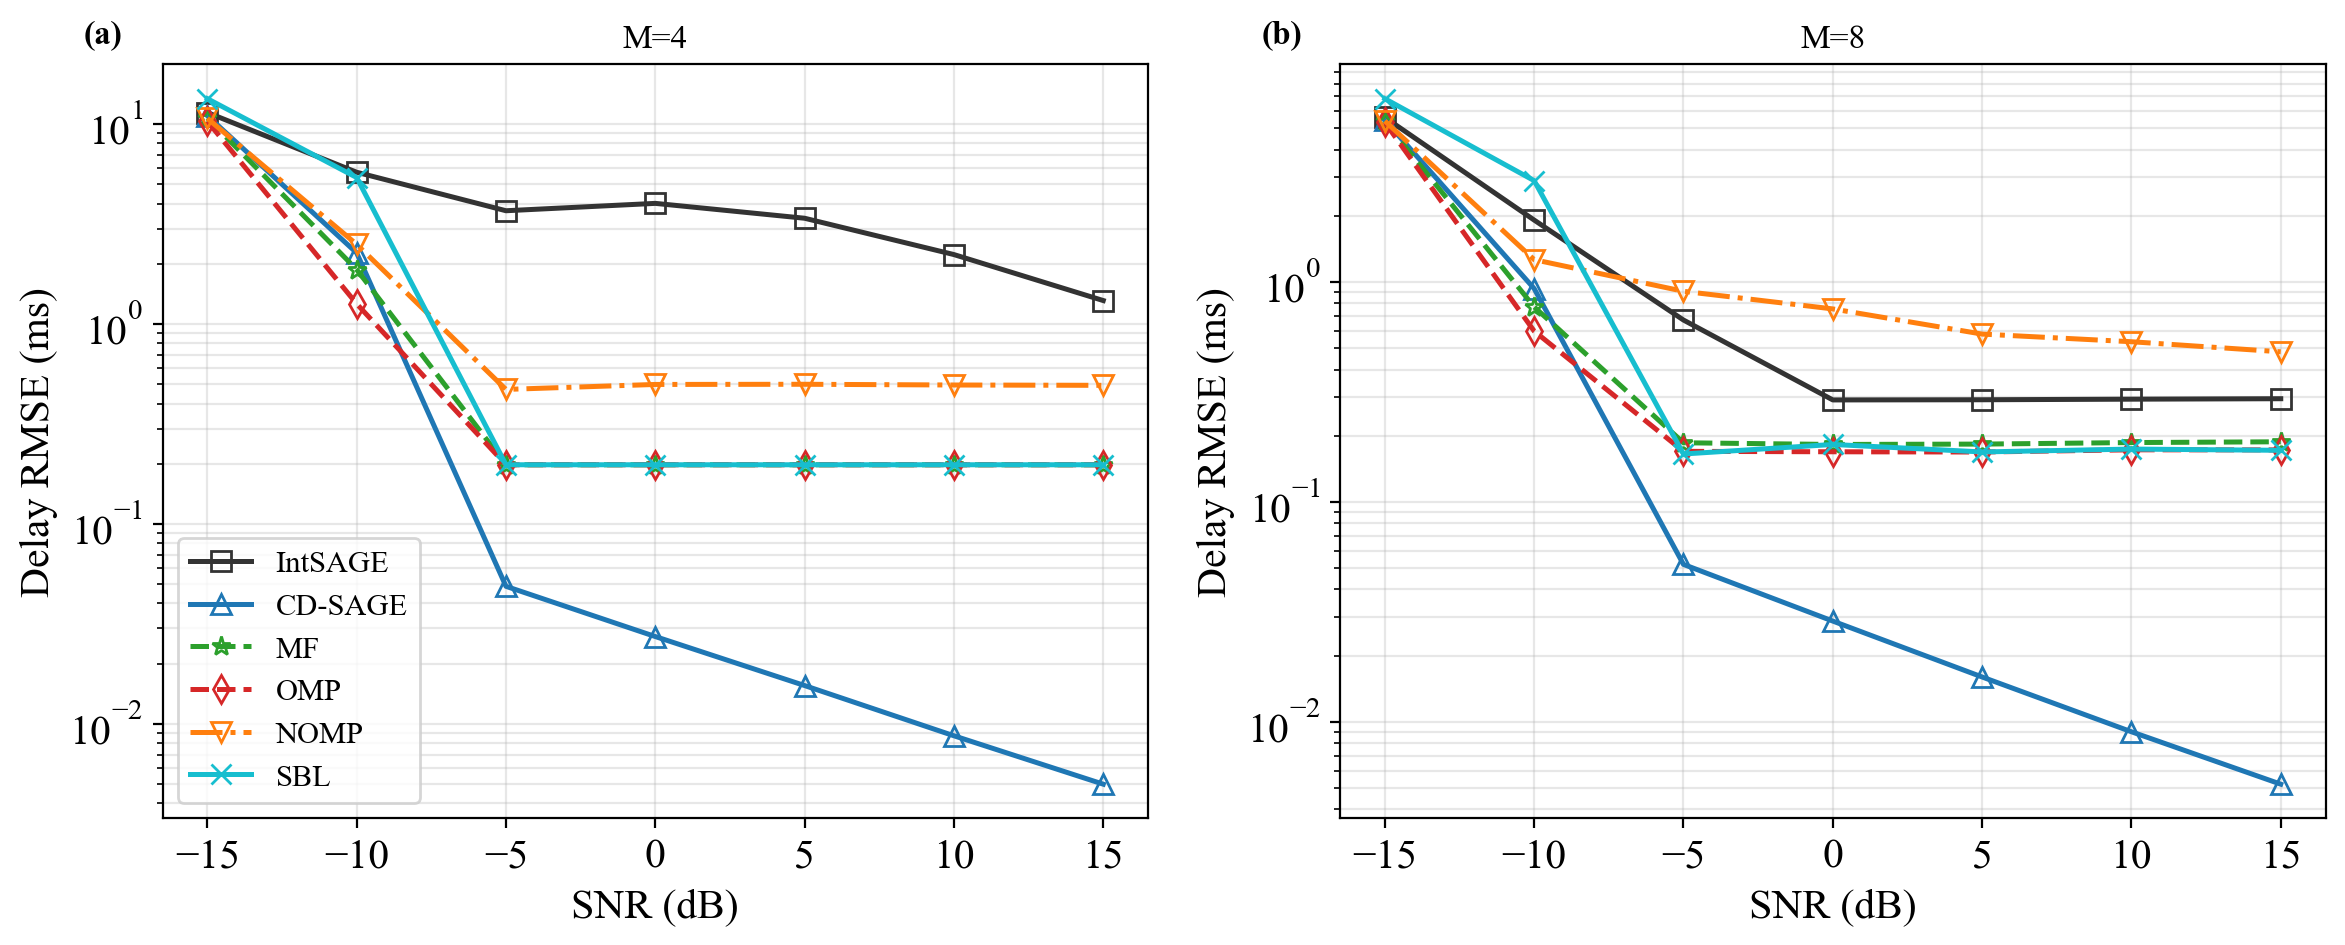
\includegraphics[width=.9\textwidth]{figs/Fig_13.png}
\caption{Delay RMSE vs.\ SNR on the Watermark NOF1 benchmark for decimation factors $M=4$ and $M=8$ (800 MC trials per SNR point).}
\label{fig:watermark}
\end{figure*}

Fig.~\ref{fig:watermark} and Table~\ref{tab:wm} present the results. Three regimes are clearly visible:

\textbf{Low SNR ($-15$ to $-10$~dB):} All algorithms are noise-dominated with comparable RMSE. No method can overcome the thermal noise floor.

\textbf{Transition ($-5$~dB):} CD-SAGE sharply transitions to near-CRB performance (RMSE $\approx 0.05$ at $M=4$), while dictionary methods (MF, OMP, SBL) immediately hit the $0.5\ T_s$ grid-quantization floor at $\sim$0.17--0.20 ms, and Int~SAGE remains limited by path masking.

\textbf{High SNR ($0$ to $+15$~dB):} CD-SAGE continues tracking the CRB (RMSE $0.027 \to 0.005$ at $M=4$), while all other algorithms exhibit flat floors independent of SNR. The dictionary methods' RMSE of 0.17--0.20 matches the theoretical quantization floor $\Delta/\sqrt{12} \approx 0.144$ for a $0.5\ T_s$ grid, with the excess attributable to residual inter-path interference.

\begin{table*}[cols=8,pos=h]
\centering
\caption{Delay RMSE at Representative SNR --- Watermark NOF1 (800 MC trials/SNR)}
\label{tab:wm}
\footnotesize
\begin{tabular}{@{}ccrrrrrr@{}}
\toprule
$M$ & SNR (dB) & Int SAGE & \textbf{CD-SAGE} & MF & OMP & NOMP & SBL \\
\midrule
\multirow{3}{*}{4} & $-5$  & 3.847 & \textbf{0.049} & 0.198 & 0.198 & 0.494 & 0.198 \\
                    & $0$   & 4.012 & \textbf{0.027} & 0.198 & 0.198 & 0.498 & 0.198 \\
                    & $+15$ & 1.810 & \textbf{0.005} & 0.198 & 0.198 & 0.496 & 0.198 \\
\midrule
\multirow{3}{*}{8} & $-5$  & 0.669 & \textbf{0.052} & 0.186 & 0.170 & 0.764 & 0.186 \\
                    & $0$   & 0.291 & \textbf{0.029} & 0.183 & 0.169 & 0.755 & 0.183 \\
                    & $+15$ & 0.229 & \textbf{0.005} & 0.188 & 0.173 & 0.778 & 0.190 \\
\bottomrule
\end{tabular}
\end{table*}

\subsection{Key Findings}

\begin{enumerate}
\item \textbf{CD-SAGE is the only algorithm that tracks the CRB across all decimation factors and SNR.} At $M=4$ and \SI{0}{dB}, it achieves a \textbf{149$\times$ improvement} over Int~SAGE and a \textbf{7.3$\times$ advantage} over the best dictionary method.
\item \textbf{Dictionary methods are fundamentally bounded by grid quantization.} MF, OMP, and SBL all plateau at $\sim$0.17--0.20 ms for $\SNR \ge -5$~dB, exactly the $0.5\ T_s$ grid-quantization floor---the cleanest possible demonstration that discrete-grid methods cannot overcome the resolution limit of their dictionary.
\item \textbf{Path masking is a real phenomenon on measured channels.} At $M=4$, two decimated CIR paths fall within the same integer-grid correlation lobe, causing Int~SAGE to fail catastrophically (RMSE $\approx 4$). CD-SAGE's E-step interference cancellation resolves this masking, mirroring the Path~1/2 behavior in simulations (Section~\ref{sec:results}).
\item \textbf{The two-stage design is validated on real data.} CD-SAGE's RMSE of 0.027--0.029 at \SI{0}{dB} is nearly independent of decimation factor, confirming that continuous-delay estimation eliminates the grid-quantization floor on real, measured multipath channels.
\end{enumerate}

% ===========================================================================
% SECTION 7: CONCLUSION
% ===========================================================================
\section{Conclusion}
\label{sec:conclusion}

This paper presented a two-stage fractional delay refinement strategy for SAGE-based multipath channel estimation. Three contributions constitute the core findings:

\begin{enumerate}
\item \textbf{Theoretical Analysis:} We characterized the structural nature of the grid-mismatch error and established a complete theoretical framework for the parabolic interpolation estimator. Lemma~1 proved the $\delta$-invariance of the parabolic denominator under the idealized quadratic autocorrelation model, explaining the mechanism of near-exact recovery. Theorem~1 provided the closed-form asymptotic variance $\Var(\hat{\delta}) = (12\delta^2+1)/(16c^2 \cdot \SNR)$, establishing the $1/\SNR$ scaling that matches the CRB. Corollary~1 established the SNR-independent efficiency ratio, elevating parabolic interpolation from an empirical heuristic to a theoretically justified estimator.

\item \textbf{CD-SAGE Algorithm:} The two-stage complementary strategy combines parabolic coarse localization with local grid refinement. Stage~1 compresses the search range from the full signal length to a narrow window at constant complexity, and Stage~2 eliminates the residual bias of the quadratic approximation with fine-step search. The algorithm requires no dictionary construction, integrates directly into existing SAGE implementations, and achieves a verified 4.5$\times$ speedup through hierarchical search acceleration without accuracy loss.

\item \textbf{Systematic Validation:} We constructed a complete validation framework from synthetic simulations to real underwater acoustic channels. Monte Carlo simulations and per-path analysis revealed the distinct failure mechanisms of baseline methods, including grid quantization, path masking, and interference limitation. Ablation studies confirmed Stage~2 as the dominant accuracy contributor. Validation on the Watermark benchmark (NOF1 Norway fjord channel) established the robustness of CD-SAGE under real multipath conditions, demonstrating consistent near-CRB performance across all decimation factors.
\end{enumerate}

The practical implication is clear: \textbf{CD-SAGE eliminates the grid-quantization floor on real measured multipath channels while maintaining the computational efficiency of the SAGE framework}, making it a drop-in upgrade for any SAGE-based channel sounding system.

\textbf{Limitations and future work.} The current Newton refinement implementation, after correcting a derivative sign error and applying Hann windowing, converges stably but plateaus at $\sim$0.37~ms RMSE due to integer-grid OMP initialization limitations for closely-spaced paths. Replacing the integer-grid OMP with a dictionary-based initialization would further improve NOMP accuracy. Extension to time-varying channels with Doppler estimation and integration with deep unfolding architectures represent natural next steps.

% ===========================================================================
% APPENDIX
% ===========================================================================
\appendix
\section{Full Derivation of Theorem~1}
\label{app:theorem1}

The parabolic estimator is $\hat{\delta} = f(y_{-1}, y_0, y_{+1})$ where:
\begin{equation}
f(y_{-1}, y_0, y_{+1}) = \frac{y_{-1} - y_{+1}}{2(y_{-1} - 2y_0 + y_{+1})} \triangleq \frac{N}{2D}
\label{eq:A1}
\end{equation}
At the noiseless point, under the quadratic autocorrelation model $R(\tau) \approx 1 - c\tau^2$:
\begin{equation}
N^0 = -4c|\alpha|\delta, \quad D^0 = -2c|\alpha|
\label{eq:A2}
\end{equation}
where $D^0$ is $\delta$-invariant (Lemma~1). Substituting~\eqref{eq:A2} into~\eqref{eq:A1} yields $\hat{\delta} = (-4c|\alpha|\delta) / (2 \cdot (-2c|\alpha|)) = \delta$, confirming exact noiseless recovery.

\subsection{Gradient of \texorpdfstring{$f$}{f}}

The partial derivatives via the quotient rule, evaluated at $(N^0, D^0) = (-4c|\alpha|\delta, -2c|\alpha|)$:
\begin{equation}
g_{-1} = \frac{2\delta - 1}{4c|\alpha|}, \quad
g_0    = -\frac{\delta}{c|\alpha|}, \quad
g_{+1} = \frac{2\delta + 1}{4c|\alpha|}
\label{eq:A4}
\end{equation}
Consistency check: $g_{-1} + g_0 + g_{+1} = 0$, required for scale-invariance.

\subsection{Variance and Bias}

First-order Taylor expansion $\hat{\delta} - \delta \approx \sum_m g_m \varepsilon_m$ with independent noise perturbations $\varepsilon_m \sim \Nc(0, N_0/2)$ yields:
\begin{align}
\Var(\hat{\delta}) &\approx (g_{-1}^2 + g_0^2 + g_{+1}^2) \cdot \frac{N_0}{2} \nonumber\\
&= \frac{(2\delta-1)^2 + 16\delta^2 + (2\delta+1)^2}{16c^2|\alpha|^2} \cdot \frac{N_0}{2} \nonumber\\
&= \frac{24\delta^2 + 2}{16c^2|\alpha|^2} \cdot \frac{N_0}{2}
\label{eq:A6}
\end{align}
Substituting $\SNR = |\alpha|^2/N_0$:
\begin{equation}
\Var(\hat{\delta}) = \frac{12\delta^2 + 1}{16c^2 \cdot \SNR}
\label{eq:A7}
\end{equation}
For practical implementation, the curvature parameter $c$ in the above expressions should be replaced by the \emph{effective curvature} $c_{\text{eff}}$, obtained by evaluating the actual waveform autocorrelation $|R(\tau)|^2$ at the three sampling points and calibrating the equivalent quadratic coefficient. For the 511-point QPSK waveform used in this paper, $c_{\text{eff}} \approx 0.5c$ at typical $\delta$ values, reflecting the fact that the quadratic model overestimates the autocorrelation decay at $|\tau|\approx 1$. With this calibration, the predicted variance aligns with the experimental measurements in Section~\ref{sec:results}.

With Stage~2 local grid refinement (step $\Delta = 0.005$), the total variance becomes:
\begin{equation}
\Var(\hat{\tau}_l) \approx \min\!\left( \frac{12\delta^2 + 1}{16c^2 \cdot \SNR}, \; \frac{\Delta^2}{12} \right)
\label{eq:A9}
\end{equation}
At $\SNR \ge 5$~dB, the first term dominates. The quantization floor $\Delta^2/12 \approx 2.1 \times 10^{-6}$ becomes active only at $\SNR > 50$~dB, well beyond practical concern.




% Uncomment and use as the case may be
%\begin{theorem} 
%\end{theorem}

% Uncomment and use as the case may be
%\begin{lemma} 
%\end{lemma}

%% The Appendices part is started with the command \appendix;
%% appendix sections are then done as normal sections
%% \appendix



% To print the credit authorship contribution details
\printcredits

%% Loading bibliography style file
\bibliographystyle{cas-model2-names}

% Loading bibliography database
\bibliography{paper_refs}

% Biography
%\bio{}
% Here goes the biography details.
%\endbio

%\bio{pic1}
% Here goes the biography details.
%\endbio

\end{document}

